\documentclass[12pt]{article}
\usepackage[margin=1in]{geometry}
\usepackage{graphicx}
\usepackage{amsmath}
\usepackage{hyperref}
\usepackage{appendix}
\usepackage{color}
\usepackage{multicol}

\title{\huge \bf Quick Write-up on Displaced-Vertex Muon-Groups}
\author{Jim Pivarski}

\definecolor{darkred}{rgb}{0.75,0.,0.}
\newcommand{\fixme}[1]{\textcolor{darkred}{\bf FIXME: #1}}
\newcommand{\s}[1]{{\mbox{\scriptsize #1}}}

\begin{document}
\maketitle

\section{Intro}

I'm really glad that you're interested in studying this channel--- I
had only been studying it because I wanted to be sure that the
muon-group infrastructure I was developing would not unnecessarily
reject groups of muons if they are displaced from the beamline.  There
are good reasons to expect hidden-valley models to produce di-muons or
multi-muons with displaced vertices: the key aspect of these models is
that the dark bosons are only weakly coupled to the Standard Model,
which can be pushed to the extreme of making the dark bosons
metastable.  Figure~\ref{fig:strassler} shows an example from a
realistic model.

\begin{figure}[h]
\begin{center}
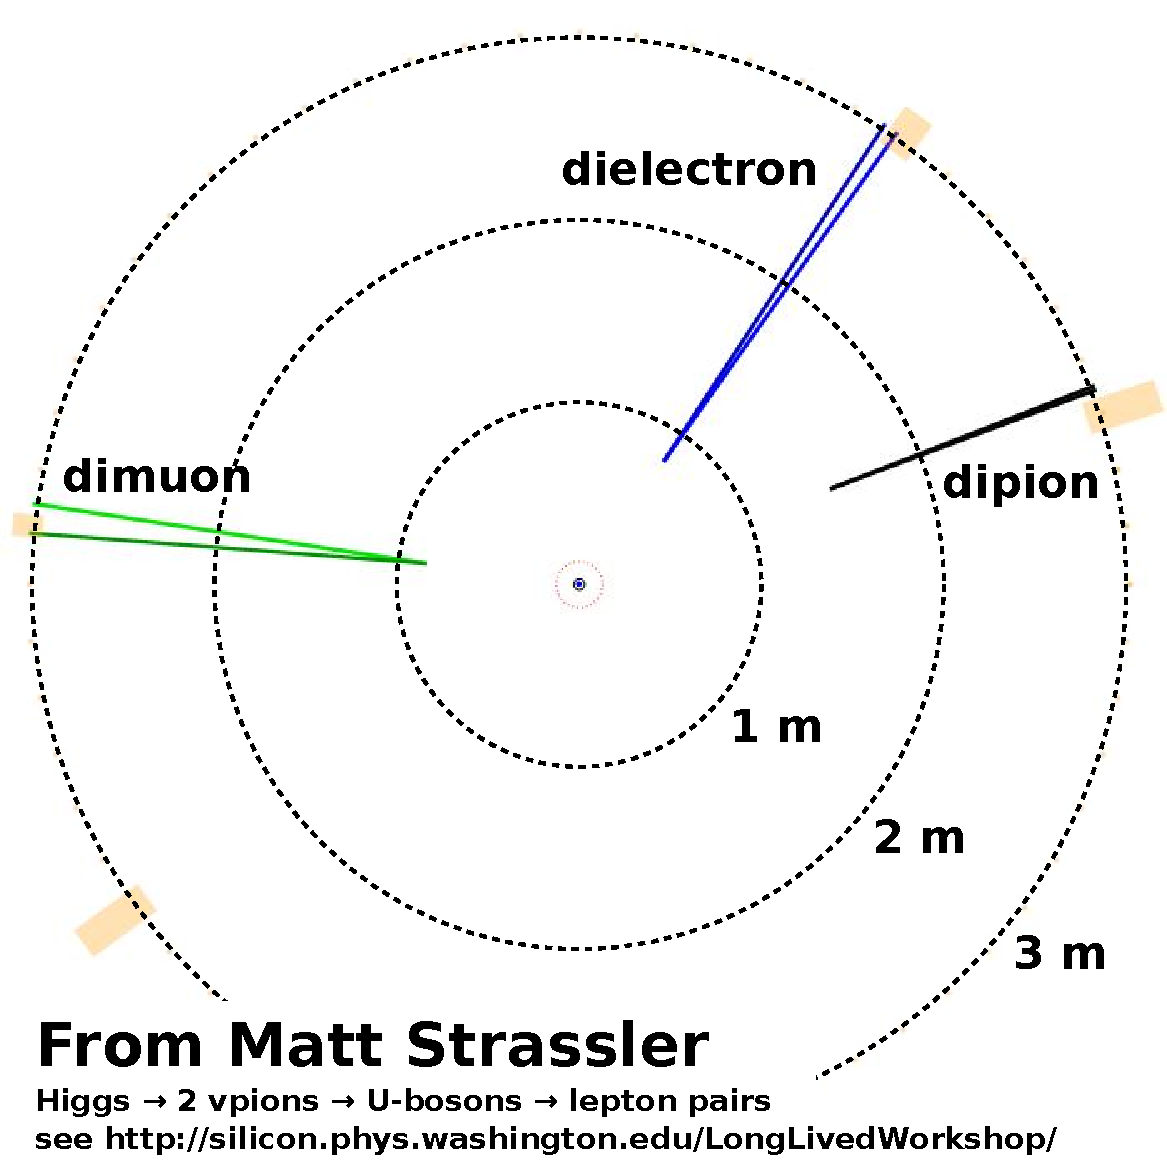
\includegraphics[width=0.5\linewidth]{fig/displaced_vertex_mugroups/leptjets1e.pdf}
\end{center}

\caption{Event display from a hidden valley model in a PGS simulation
  (see Ref.~\cite{strassler}). \label{fig:strassler}}
\end{figure}

\pagebreak
Moreover, the Standard Model provides some nice targets to show that
your analysis is working.  There's a (very rare) resonance peak from
$K_L \to \mu^+\mu^-$ ($\mathcal{B} = 6\times 10^{-9}$); it might be
worth checking the efficiency-corrected yield of $K_S$ to see if this
would ever be feasible.  Even if the peak is too small, there would be
a smear at lower masses from $K_L \to \mu^+\mu^- \gamma$ and
$\mu^+\mu^- \gamma\gamma$ with a few orders of magnitude higher
branching fraction ($\mathcal{B} = 10^{-7\mbox{-}8}$).  If that, also,
is too rare to see, well at least it won't be a background.  Also,
photon conversion can result in di-muons\cite{geant}, so you may be
able to see the pixel detector supports in the vertex distribution,
just as you would in the di-electron channel (with a much higher rate).

I'm writing up what I know about this channel in the hope that it will
be useful for you.  Afterward, I'll focus on the prompt pairs of
muon-groups: I'm just glad that this important channel won't be
ignored.  (When I suggested that we work on different signatures which
could have qualitatively different issues, this was one of the four.)

\section{Range of sensitivity}

I checked out-of-the-box Monte Carlo efficiencies for this channel,
and show them as two of the curves in Fig.~\ref{fig:acceptance1}.
Since then, I learned that there are major reasons to be suspicious of
the Monte Carlo trigger simulation, particularly in the endcap (there
are even L1 algorithms that were not propagated into the L1Emulator
until a very recent CMSSW release).  Nevertheless, what we see in the
figure (CMSSW\_3\_6\_3) makes qualitative sense:
\begin{itemize}
\item L1 is not very sensitive to the distance of the di-muon from the
  beamline ($v_{xy}$);
\item HLT\_Mu5 is, and that's (presumably) because this HLT algorithm
  requires a StandAloneMuon constrained to the beamspot (a
  highly-displaced StandAloneMuon with such a constraint would appear
  to be curved like a low-momentum muon).
\end{itemize}

\begin{figure}
\begin{center}
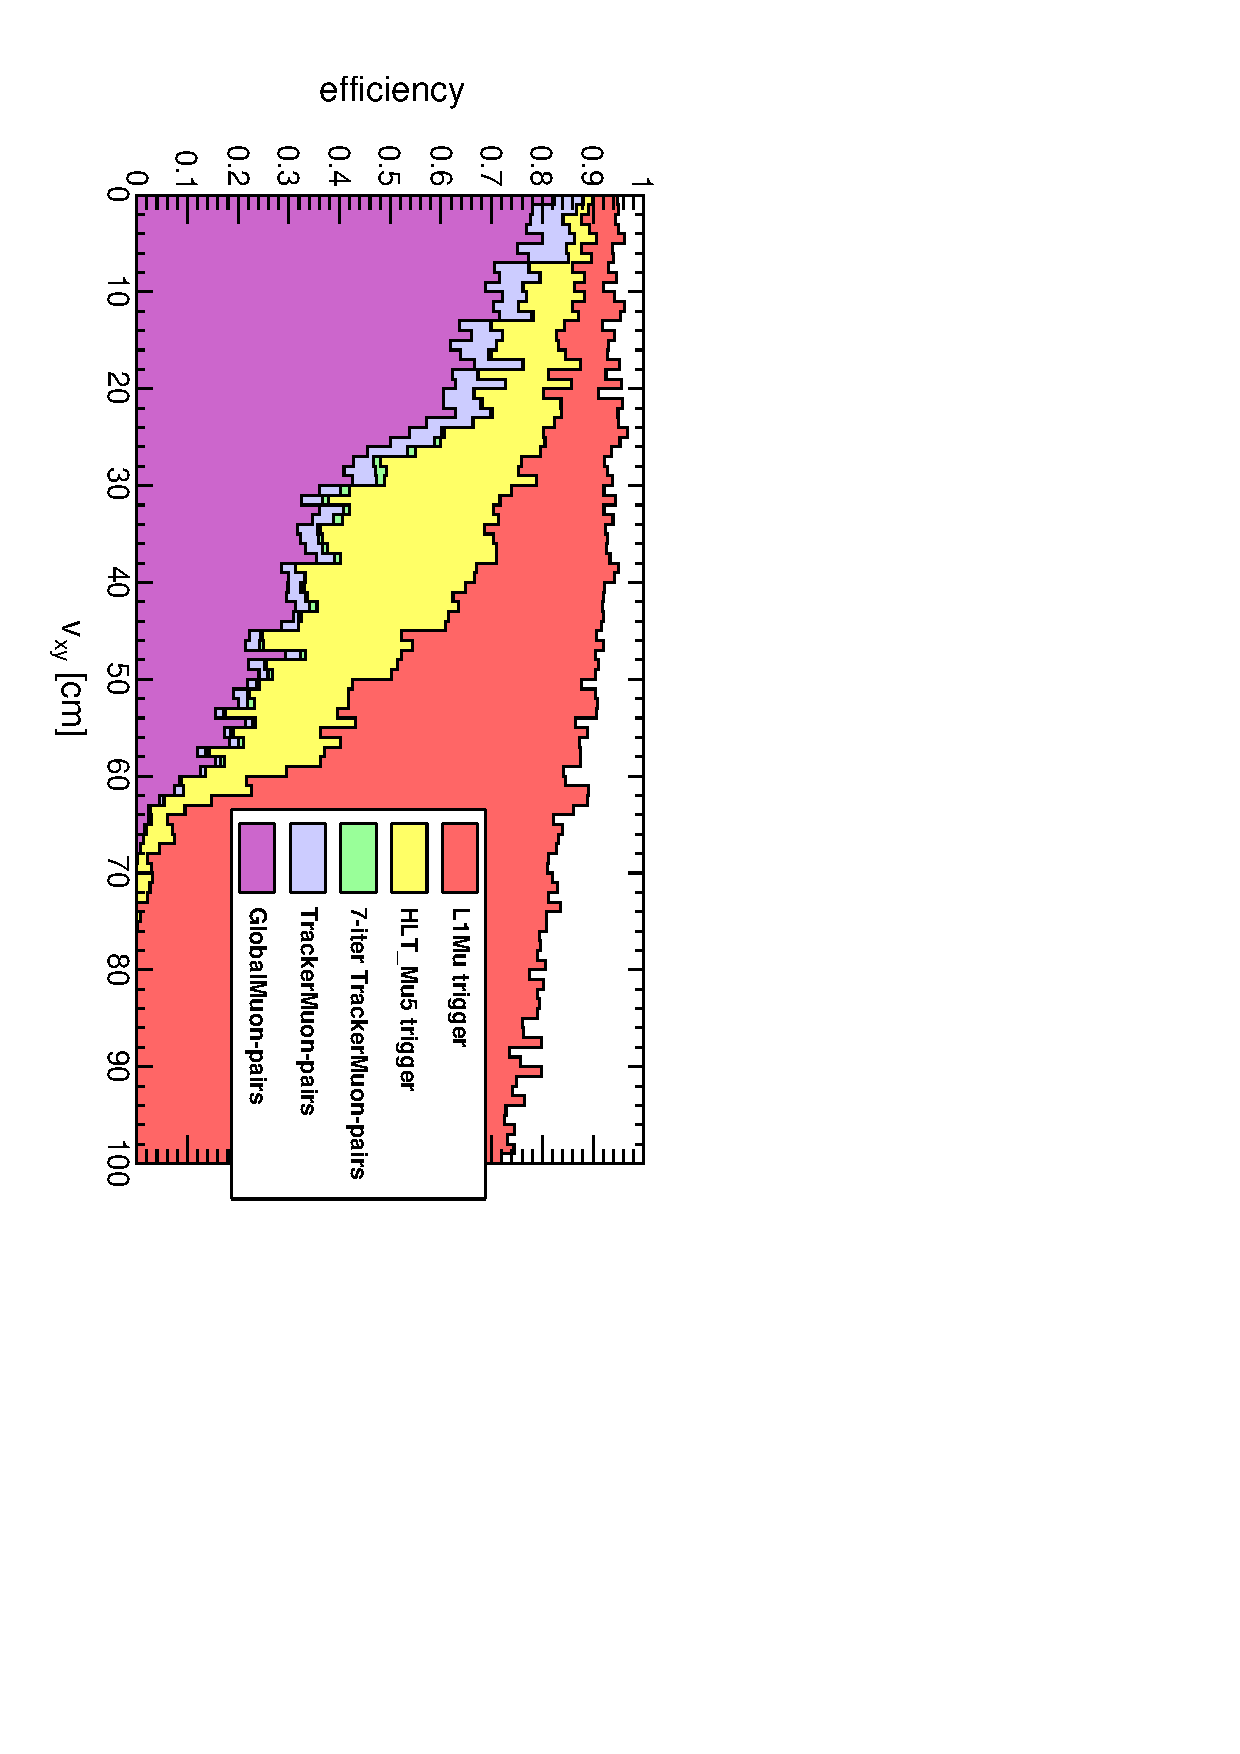
\includegraphics[height=0.8\linewidth, angle=90]{fig/acceptance5_plot/dispvert.pdf}
\end{center}

\caption{Efficiency of triggers and reconstruction algorithms as a
  function of displaced vertex $v_{xy}$, for $2m_\mu < m_\s{inv} <
  5$~GeV/$c^2$ di-muons with $p_T > 5$~GeV/$c$ and $|\eta| < 2.4$ for
  each muon. \label{fig:acceptance1}}
\end{figure}

\begin{figure}
\begin{center}
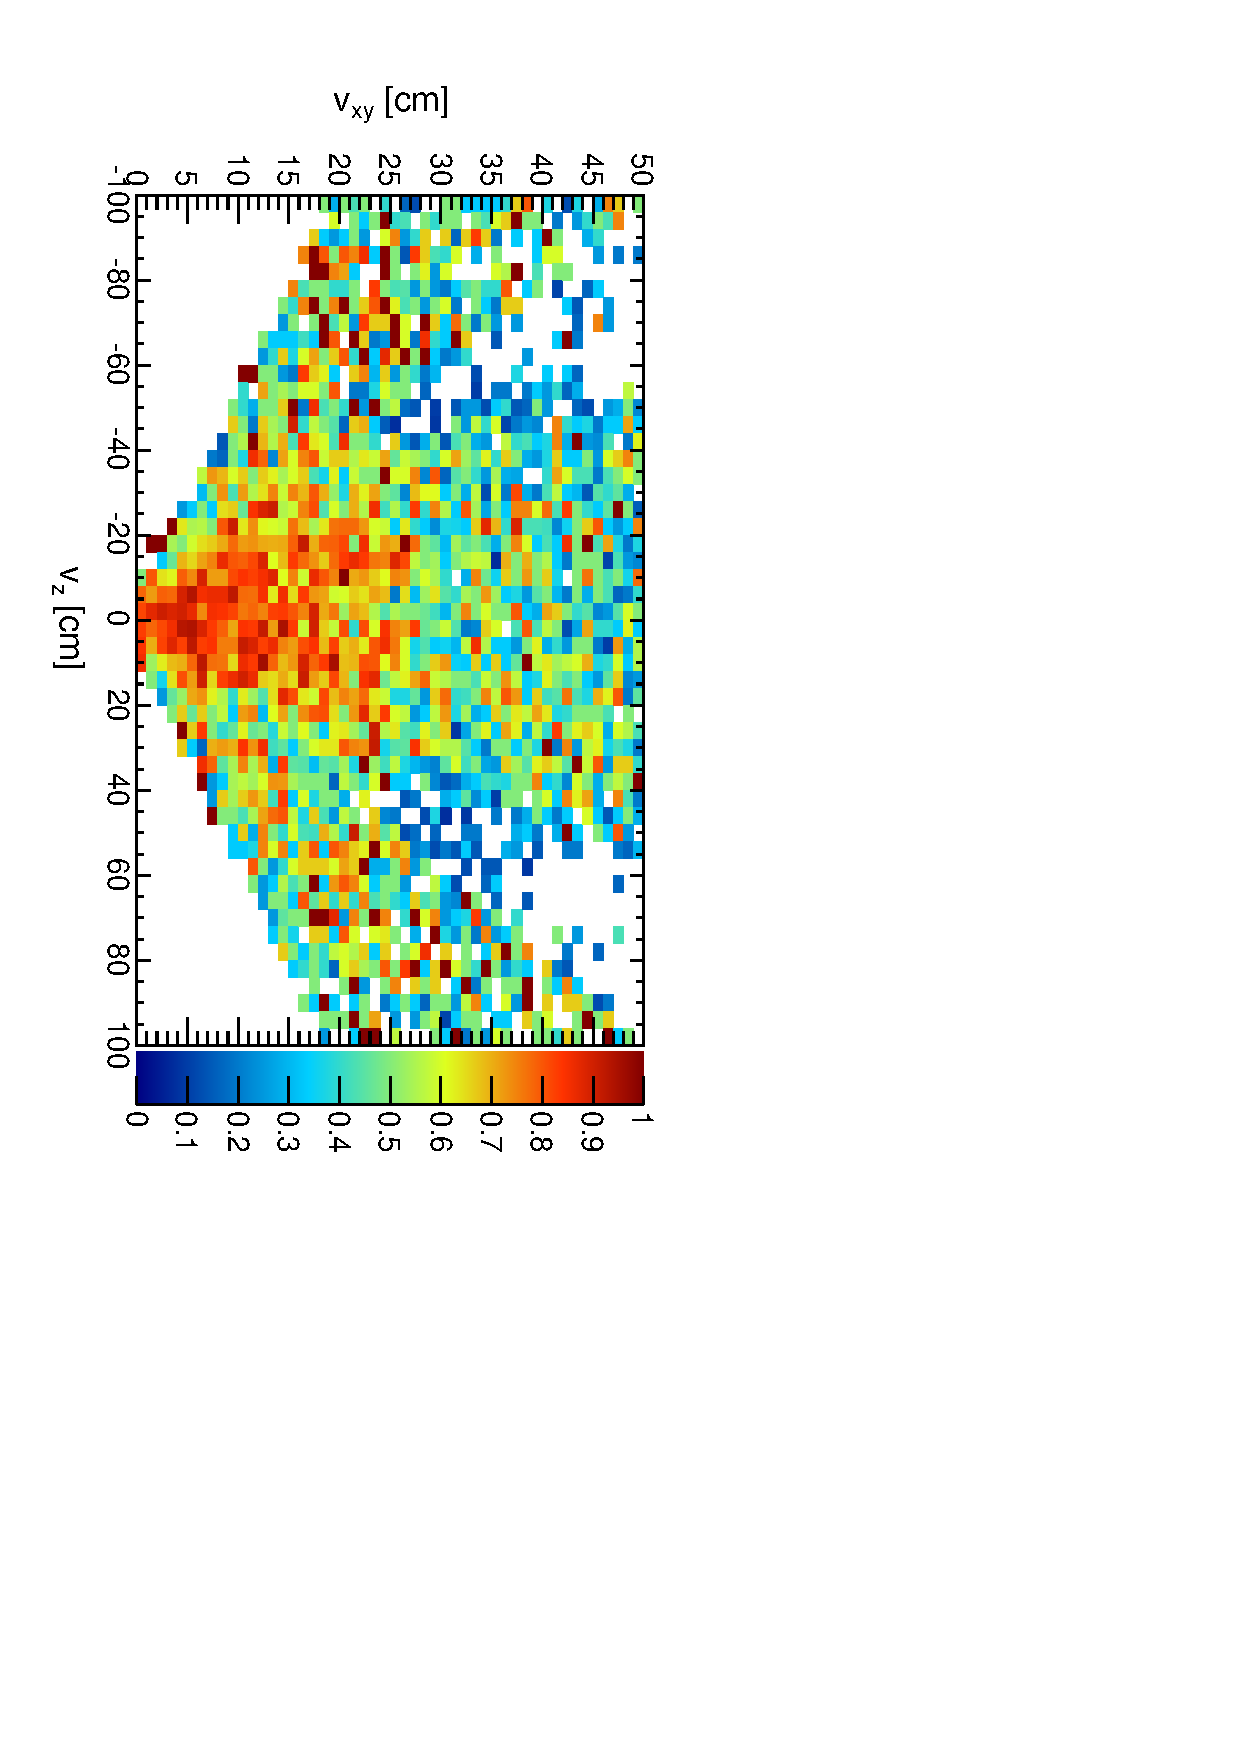
\includegraphics[height=0.8\linewidth, angle=90]{fig/acceptance5_plot/dispvert_vs_dispz.pdf}
\end{center}

\caption{Reconstruction efficiency (color scale) as a function of
  distance from the beamline $v_{xy}$ and longitudinal distance from
  the collision point $v_z$, same denominator as
  Fig.~\ref{fig:acceptance1}.  Some of the projective structure of the
  muon system (or tracker?) can be
  seen. \label{fig:dispvert_vs_dispz}}
\end{figure}

Thus, the trigger sets a limit on $v_{xy}$ acceptance at about 60~cm.
From a technical point of view, this could easily be loosened: just
add an HLT trigger without the beamspot constraint in the
StandAloneMuon fit.  However, adding a trigger requires a long-term
commitment to study and monitor the trigger--- not a small investment.

Reconstruction efficiency similarly cuts off at about 60~cm, though
for a different reason.  At some level in TrackerMuon and GlobalMuon
reconstruction, at least 8 valid hits are required from the tracker (not
strictly, but there is some cut at some level: see
Fig.~\ref{fig:tkhits}).  At high $v_{xy}$, the number of tracker hits
necessarily decreases as the muons range out of the tracker.

\begin{figure}
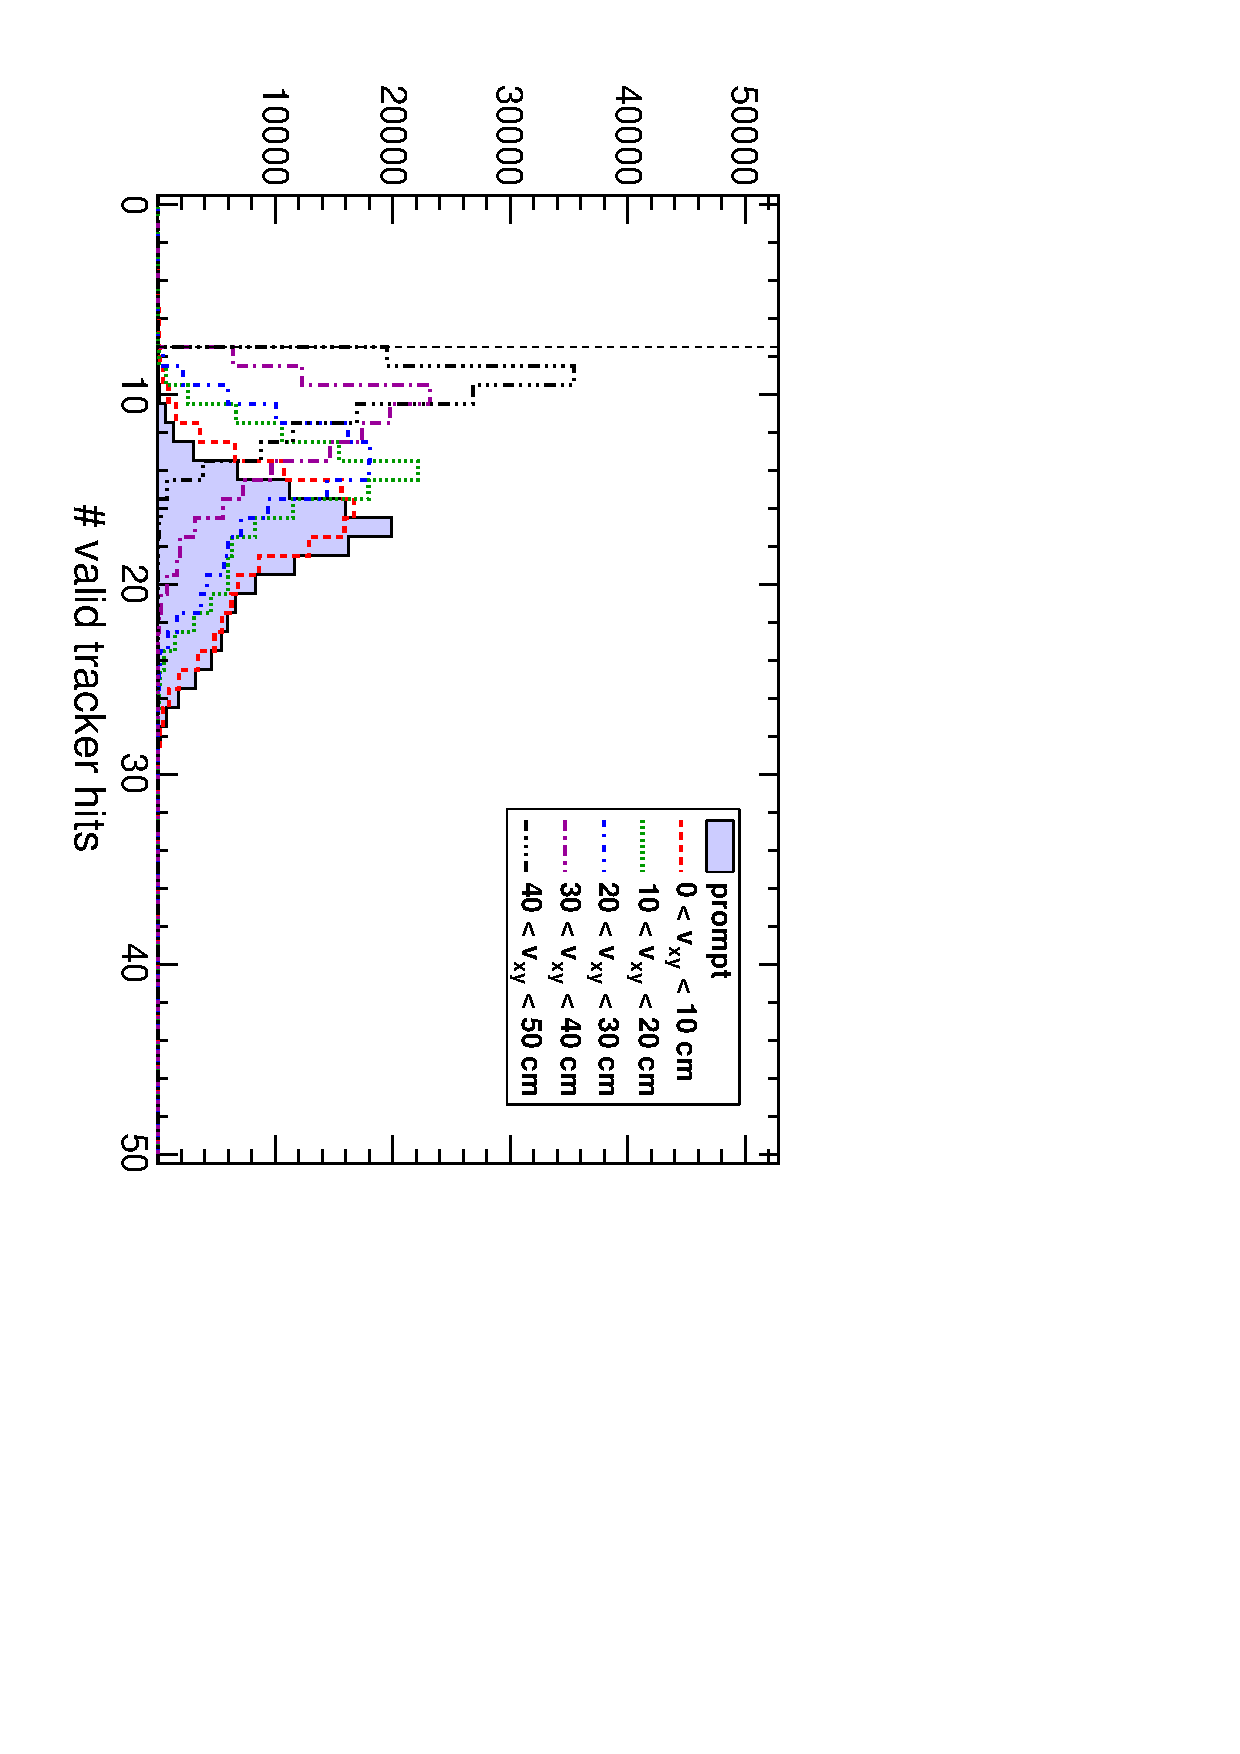
\includegraphics[height=0.49\linewidth, angle=90]{fig/backgrounds3_plot/trackslinear_tkhits.pdf}
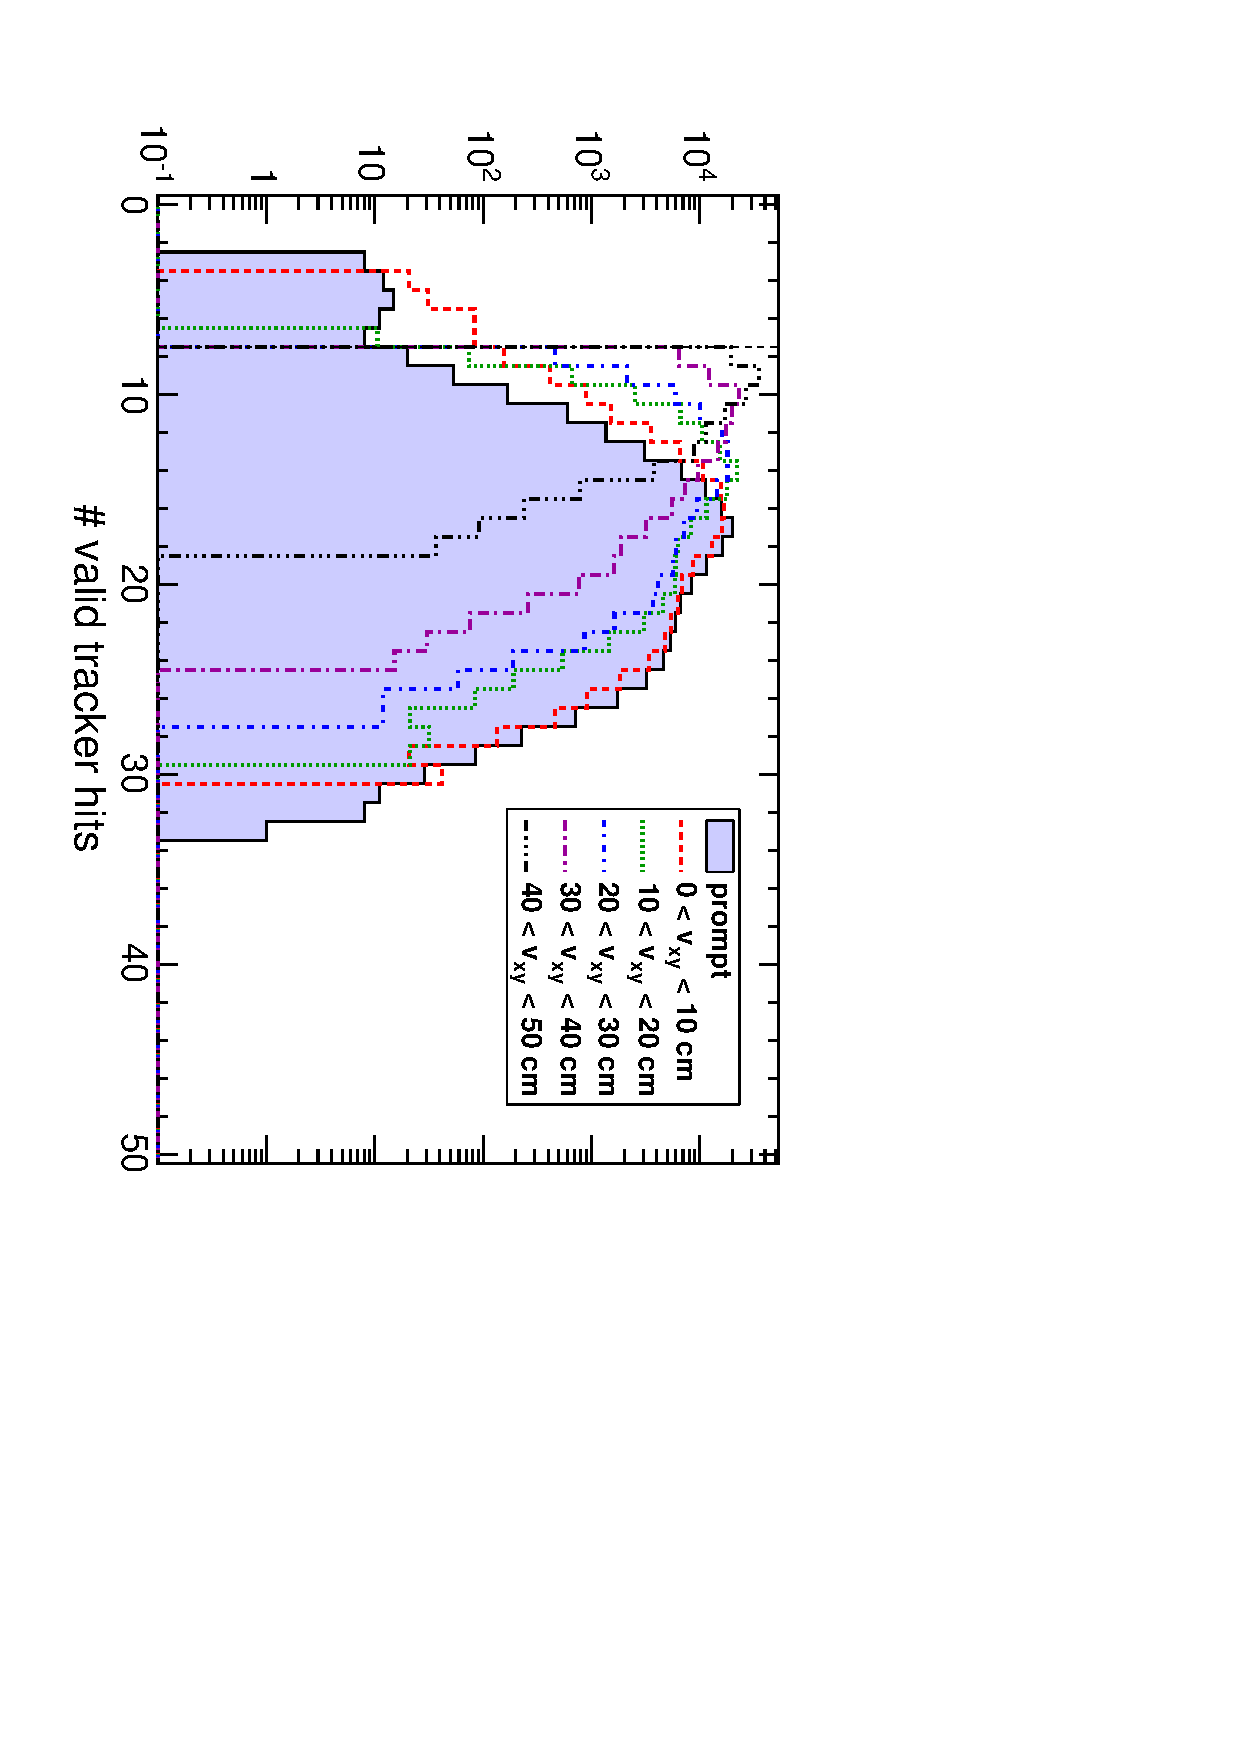
\includegraphics[height=0.49\linewidth, angle=90]{fig/backgrounds3_plot/trackslog_tkhits.pdf}

\caption{Distribution of valid tracker hits for prompt di-muons
  (filled) and displaced di-muons (open lines); each distribution is
  normalized to the same area; linear scale on left, log scale on
  right.  No explicit cut was placed at analysis level, but something
  in TrackerMuon reconstruction requires at least 8
  hits. \label{fig:tkhits}}
\end{figure}

The third reconstruction option, with very slightly more efficiency
than TrackerMuons, is TrackerMuons with conversions-like
reconstruction~\cite{conversions_tracking} (an additional two
track-finding passes to look for very displaced tracks).  It doesn't
seem to help much, and that might be because it's tuned for GSF
electron tracking, or it might be because the 8-hit requirement
cuts out the good tracks that it finds, or some other reason.

Searches for highly displaced vertices with StandAloneMuons suffer
from the poor resolution of the StandAloneMuons: prompt muons smearing
into the signal region becomes a lot more significant (I looked
briefly at this, but it was so bad that I never made a finalized
plot--- sorry).

\section{TrackerMuons vs.\ GlobalMuons}

The reason we might want to be careful about GlobalMuons is that they
are inefficient when they cross in the muon system, and this
inefficiency can be hard to model (see my talks).  The TrackerMuon
alternative doesn't have this problem, and with at least two
arbitrated segments, TrackerMuons are as background-free as
GlobalMuons, for both the prompt and the displaced cases.  This is
illustrated in Fig.~\ref{fig:TrackerSegMatch2}.
Figure~\ref{fig:nsegments} shows that this cut is stable with respect
to distance from the beamline.

\begin{figure}
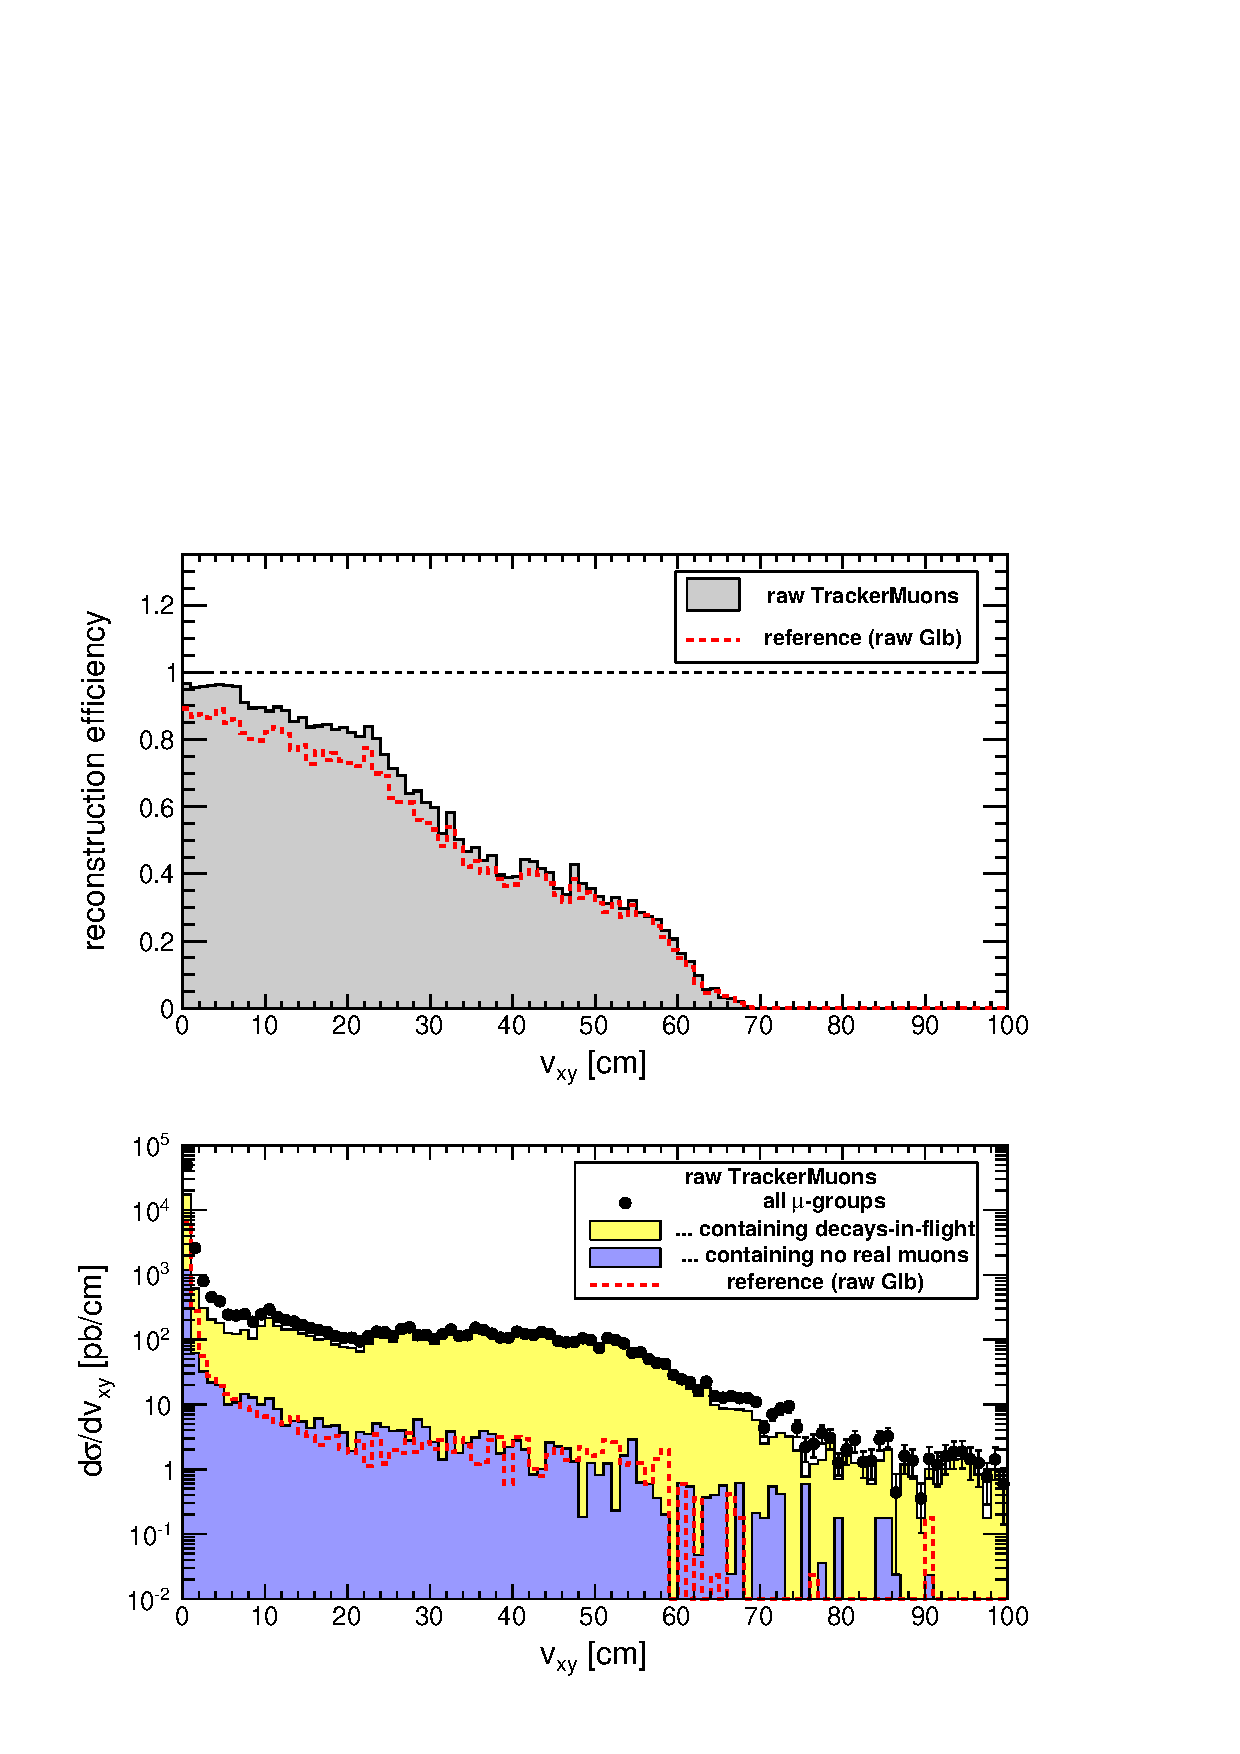
\includegraphics[width=0.49\linewidth]{fig/backgrounds3_plot/dispvert_Tracker.pdf}
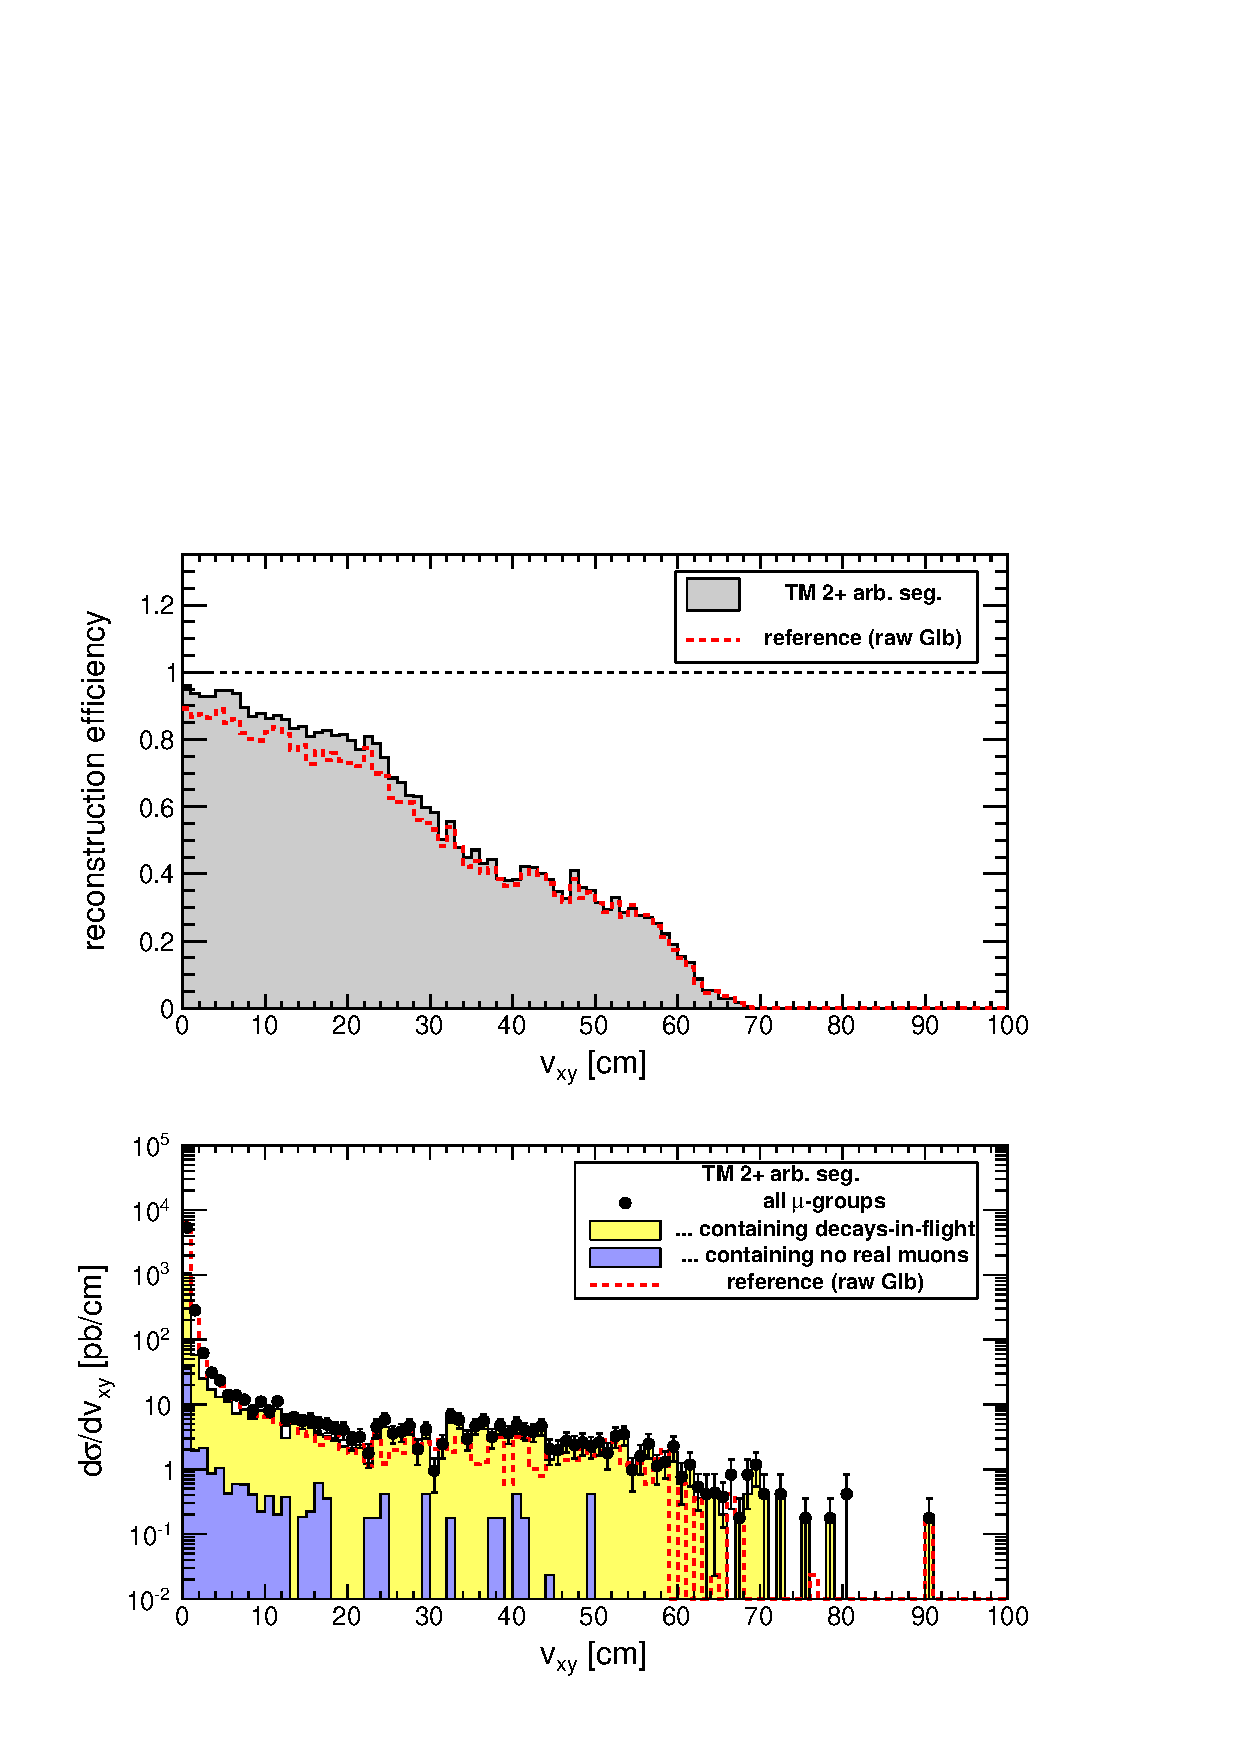
\includegraphics[width=0.49\linewidth]{fig/backgrounds3_plot/dispvert_TrackerSegMatch2.pdf}

\caption{Top: reconstruction efficiency for $2m_\mu < m_\s{inv} <
  5$~GeV/$c^2$ di-muons with $p_T > 5$~GeV/$c$ and $|\eta| < 2.4$ for
  each muon.  Bottom: InclusiveMu5\_Pt* backgrounds, colored by
  source.  Left: all TrackerMuons (GlobalMuon reference in red).
  Right: TrackerMuons with $N_\s{segments} \ge 2$ cut (same
  reference).  Background events are labeled ``decay-in-flight'' if
  one of the muons' parents was a charged pion, charged kaon, or
  strange baryon.  \label{fig:TrackerSegMatch2}}
\end{figure}

\begin{figure}
\begin{center}
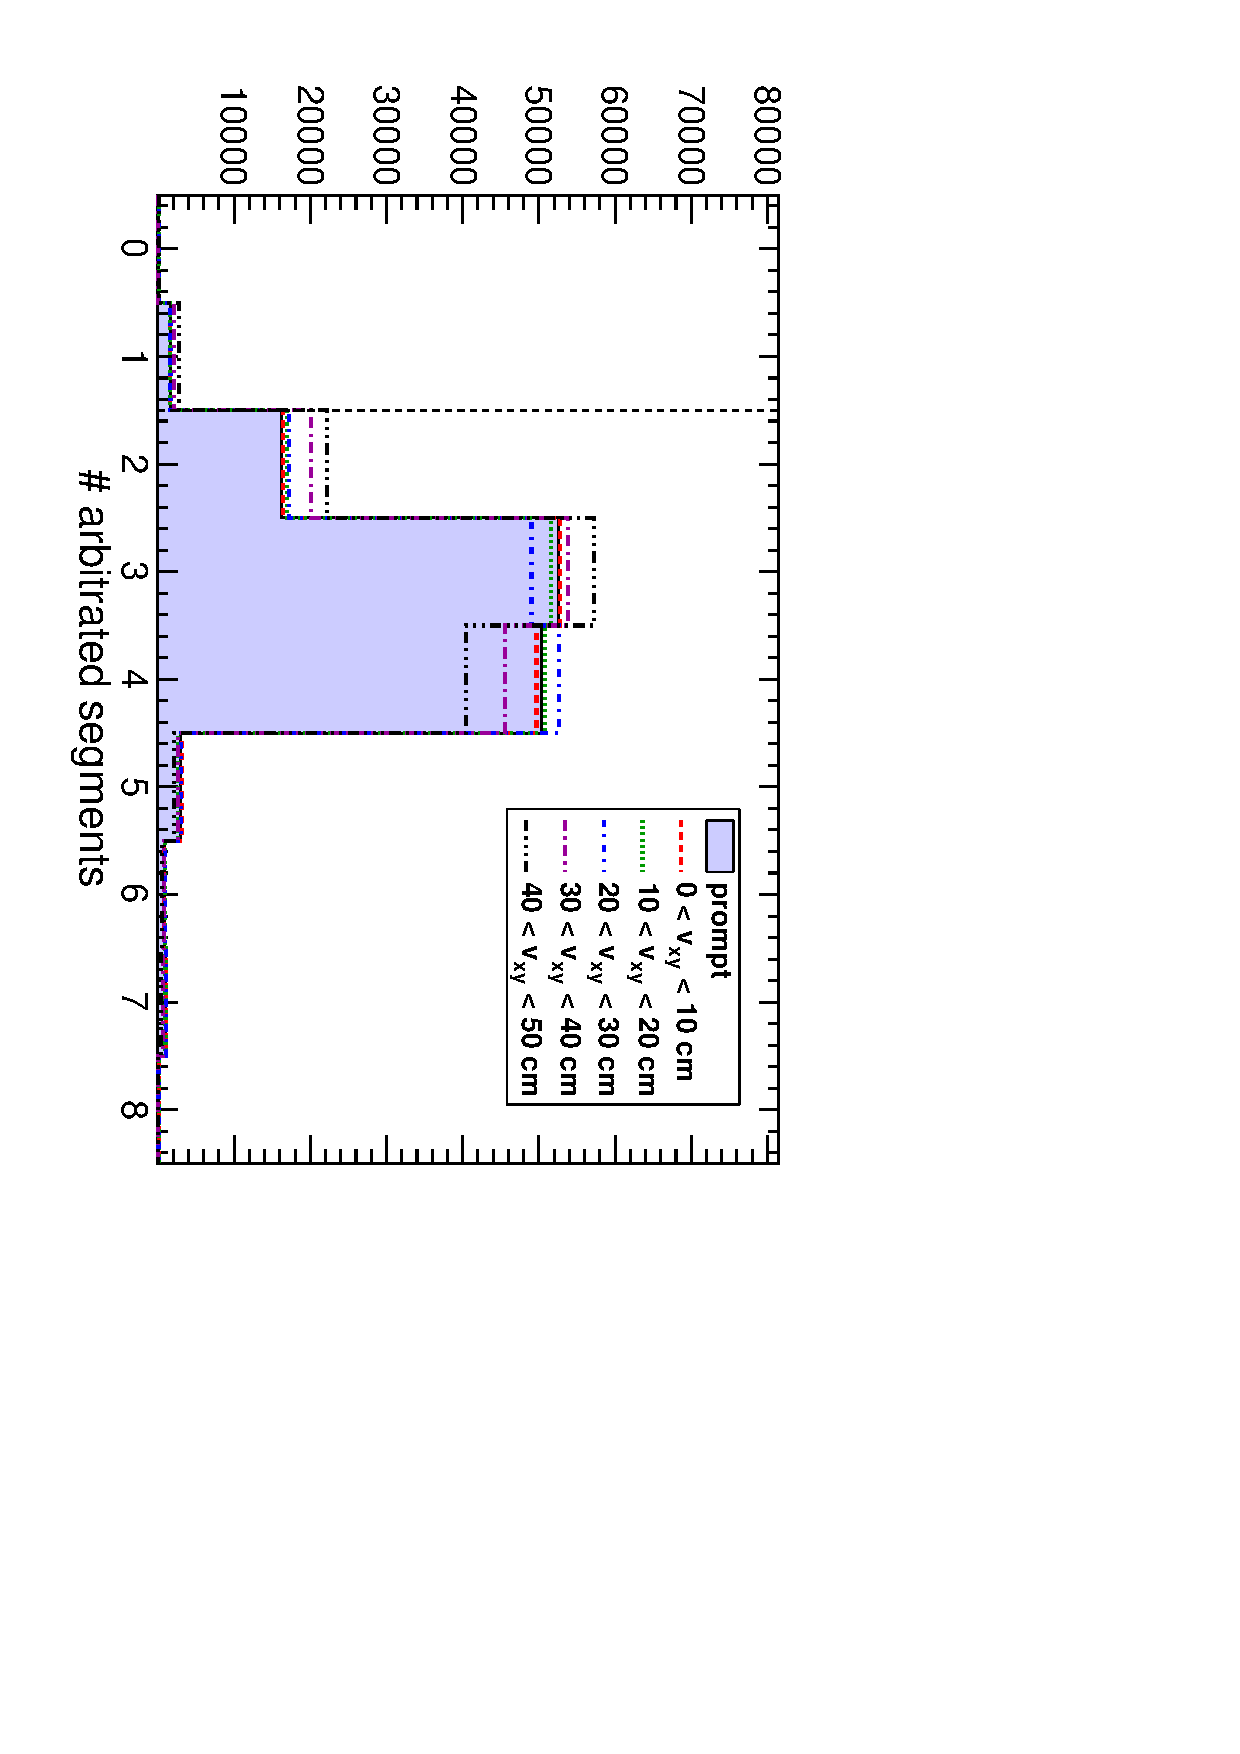
\includegraphics[height=0.49\linewidth, angle=90]{fig/backgrounds3_plot/trackslinear_segments.pdf}
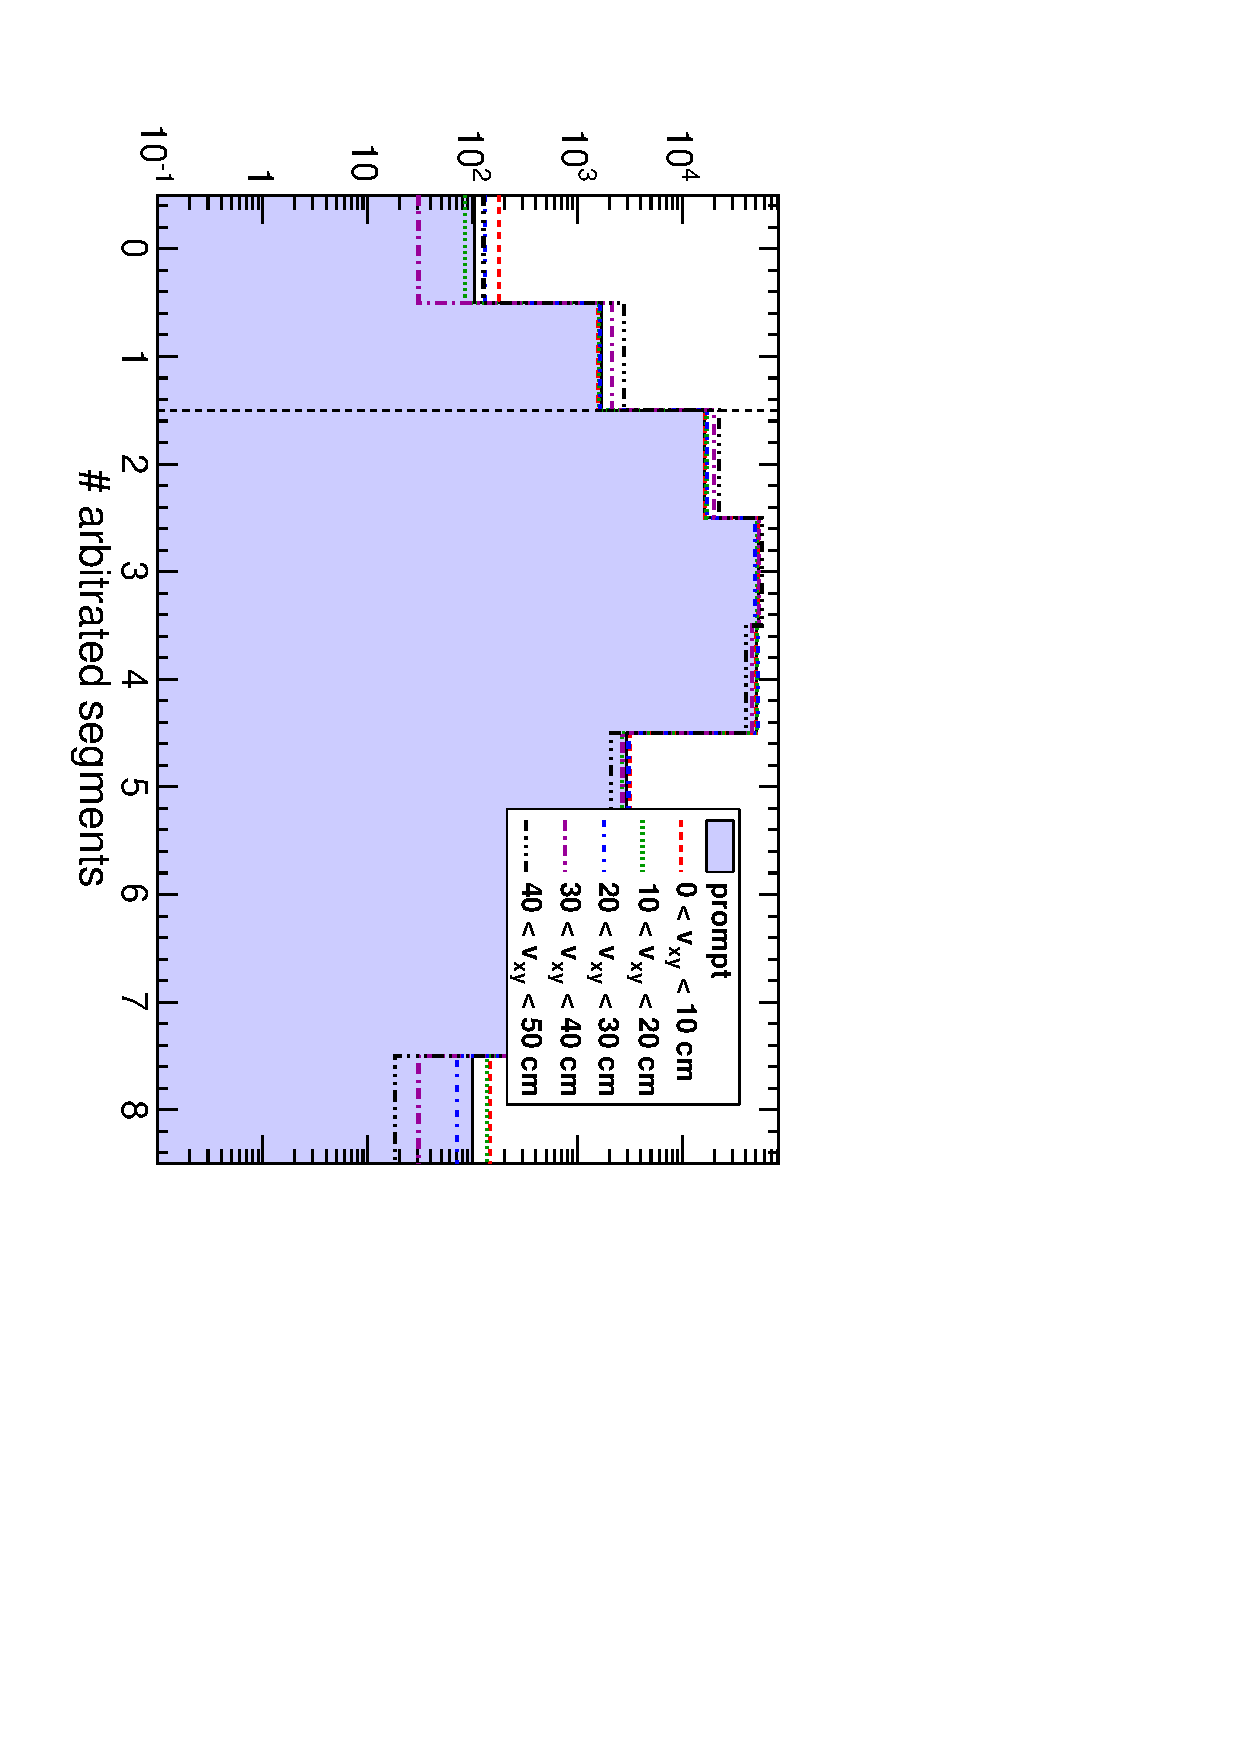
\includegraphics[height=0.49\linewidth, angle=90]{fig/backgrounds3_plot/trackslog_segments.pdf}

\caption{Number of arbitrated segments for prompt di-muons
  (filled) and displaced di-muons (open lines); each distribution is
  normalized to the same area; linear scale on left, log scale on
  right. \label{fig:nsegments}}
\end{center}
\end{figure}

\section{Other cuts}

The following cuts are stable with respect to distance from the
beamline:
\begin{itemize}
\item normalized $\chi^2$ of tracker track (Fig.~\ref{fig:normchi2})
\item uncertainty in $\phi$ parameter of tracker track (Fig.~\ref{fig:phierr})
\end{itemize}
and the following are unstable:
\begin{itemize}
\item uncertainty in $\eta$ parameter of tracker track (Fig.~\ref{fig:etaerr})
\item uncertainty in $d_{xy}$ parameter of tracker track (Fig.~\ref{fig:dxyerr})
\item uncertainty in $d_z$ parameter of tracker track (Fig.~\ref{fig:dzerr}).
\end{itemize}

All of the referenced figures show these cuts placed on TrackerMuons
with $N_\s{segments}~\ge~2$; naturally, they do the same thing to
GlobalMuons (furnished upon request).

\begin{figure}
\begin{center}
\begin{multicols}{2}
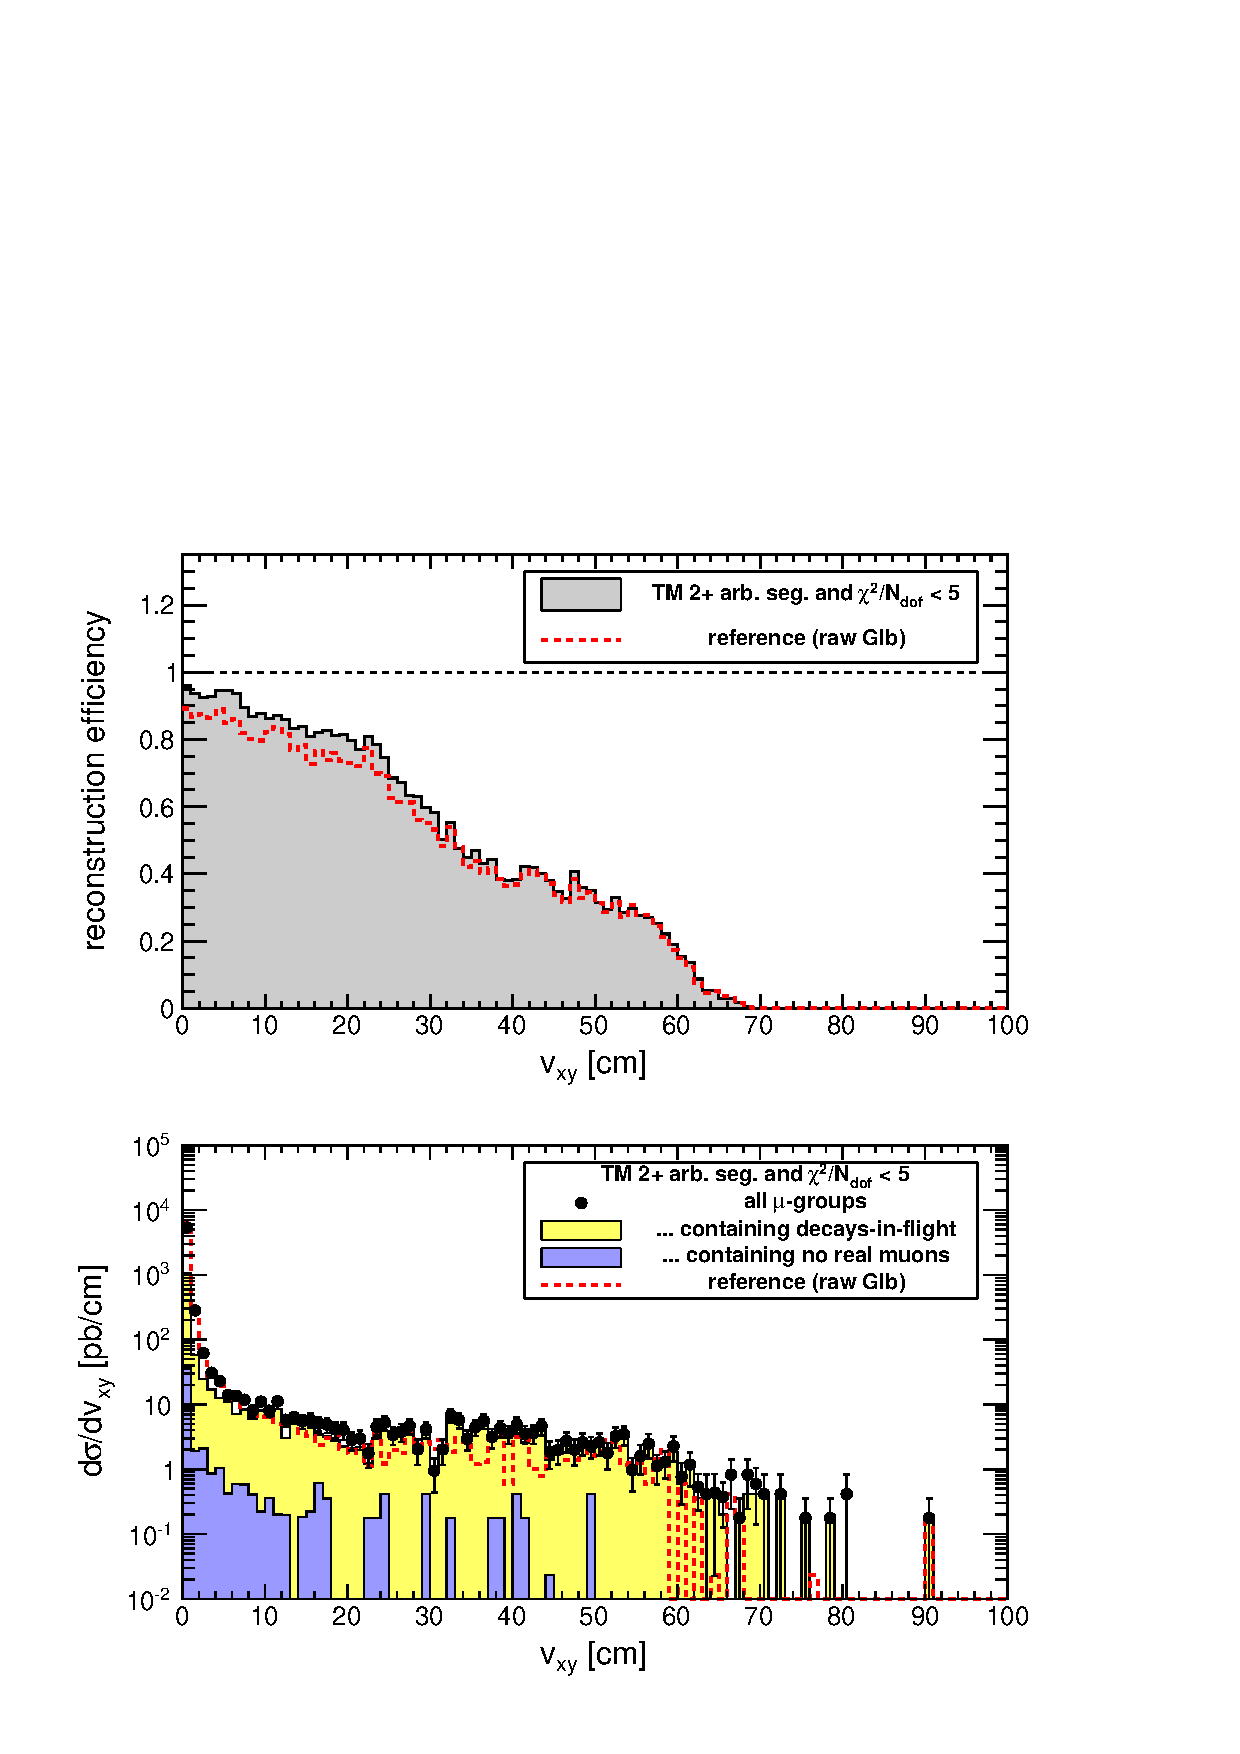
\includegraphics[width=\linewidth]{fig/backgrounds3_plot/dispvert_TrackerSegMatch2NormChi2.pdf}

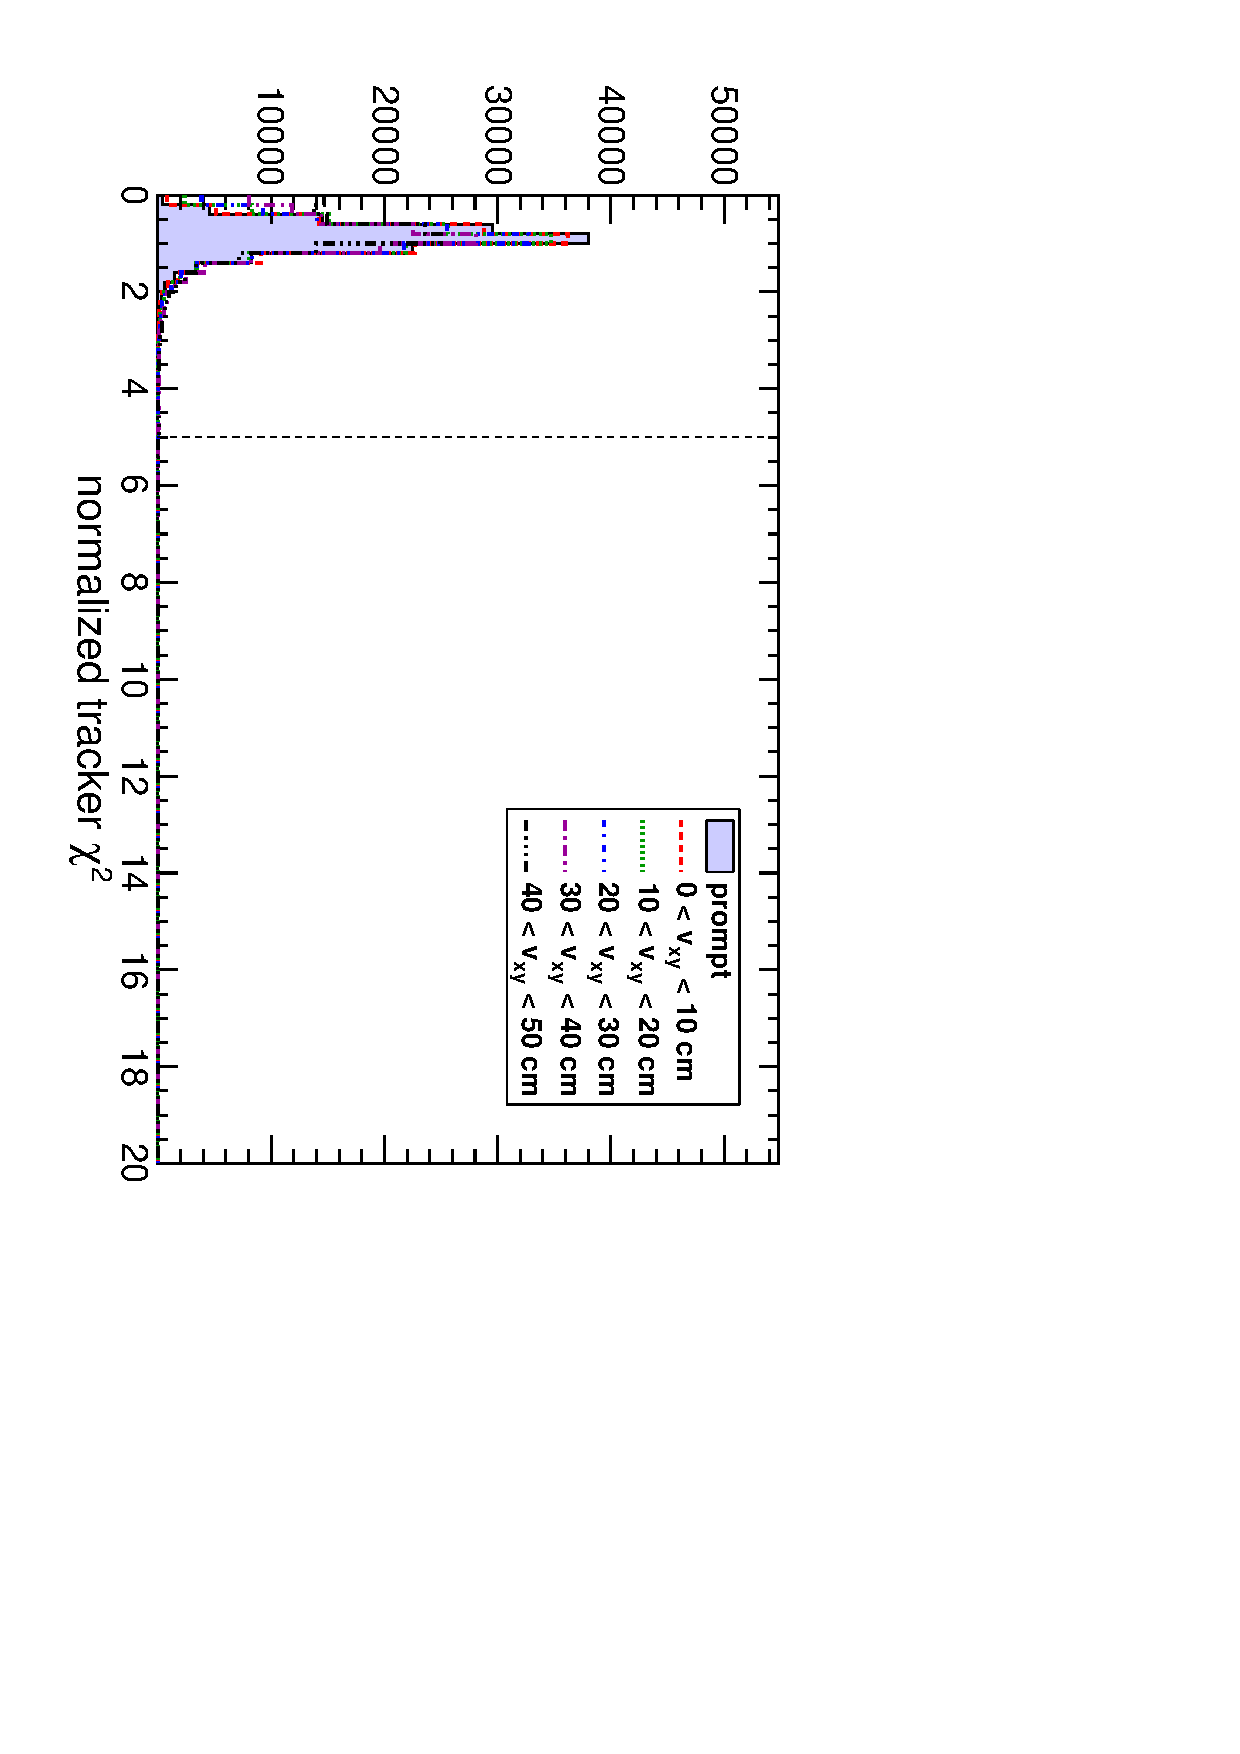
\includegraphics[height=\linewidth, angle=90]{fig/backgrounds3_plot/trackslinear_normchi2.pdf}
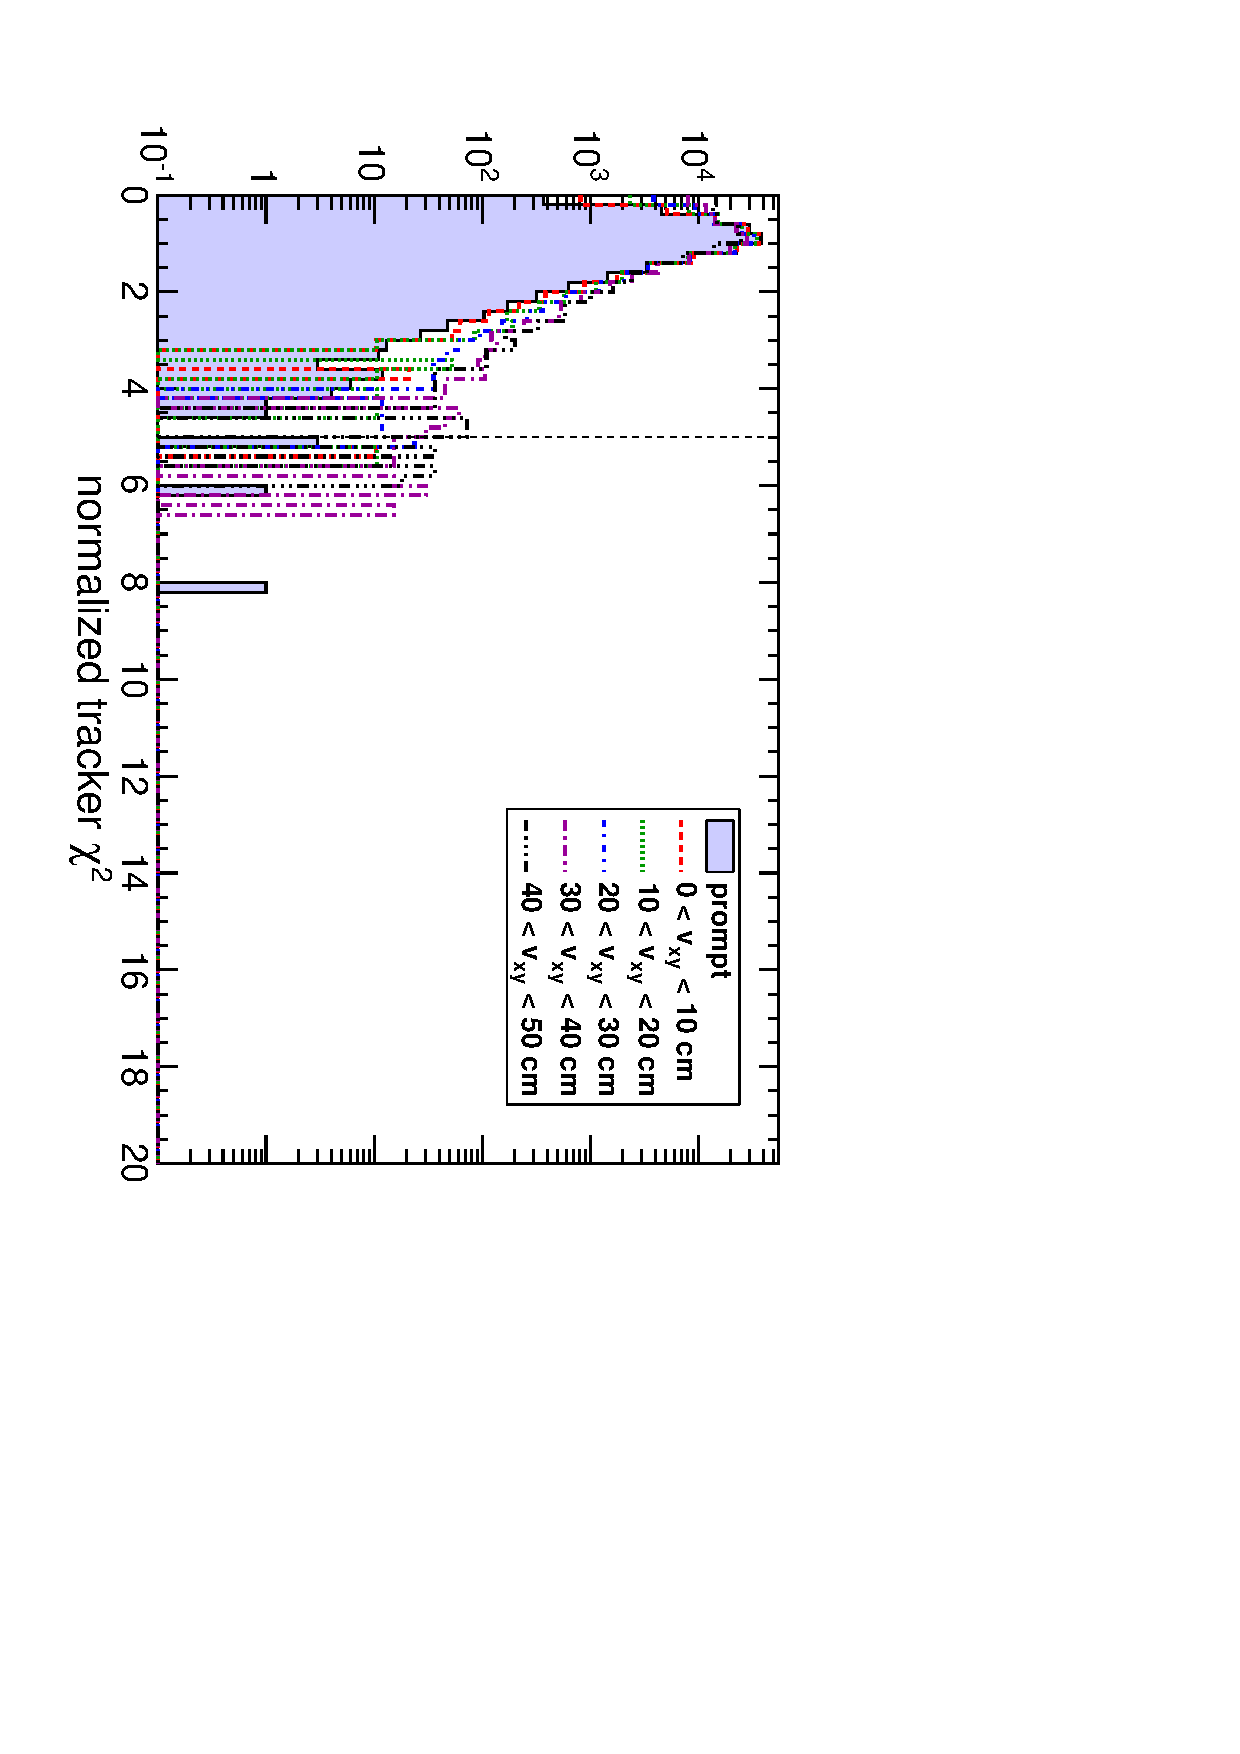
\includegraphics[height=\linewidth, angle=90]{fig/backgrounds3_plot/trackslog_normchi2.pdf}
\end{multicols}

\caption{Performance of normalized tracker $\chi^2$ cut.  Left: TrackerMuon (with $N_\s{segments}~\ge~2$) efficiency and backgrounds vs.\ $v_{xy}$ with the cut; right: linear and log distributions of the cut with the threshold indicated by a vertical line. \label{fig:normchi2}}
\end{center}
\end{figure}

\begin{figure}
\begin{center}
\begin{multicols}{2}
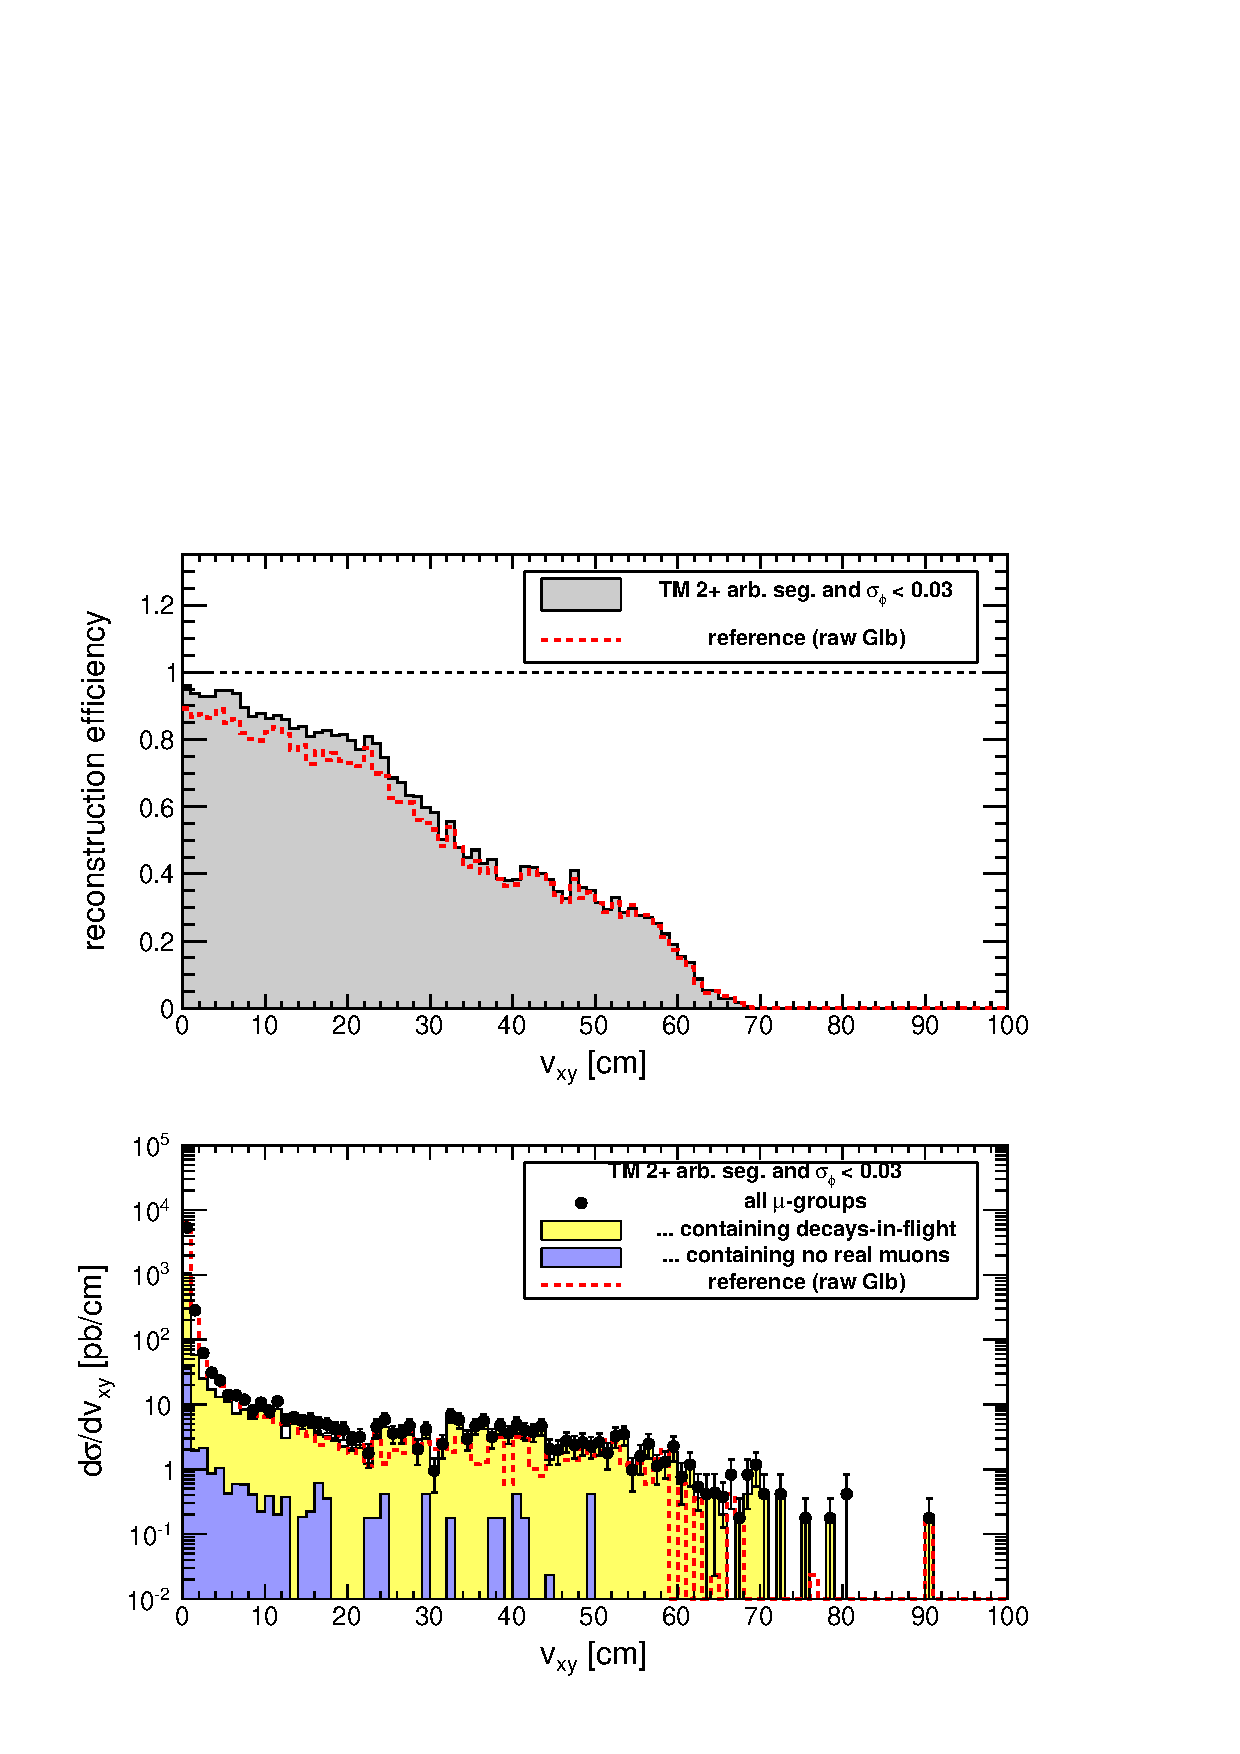
\includegraphics[width=\linewidth]{fig/backgrounds3_plot/dispvert_TrackerSegMatch2PhiErr.pdf}

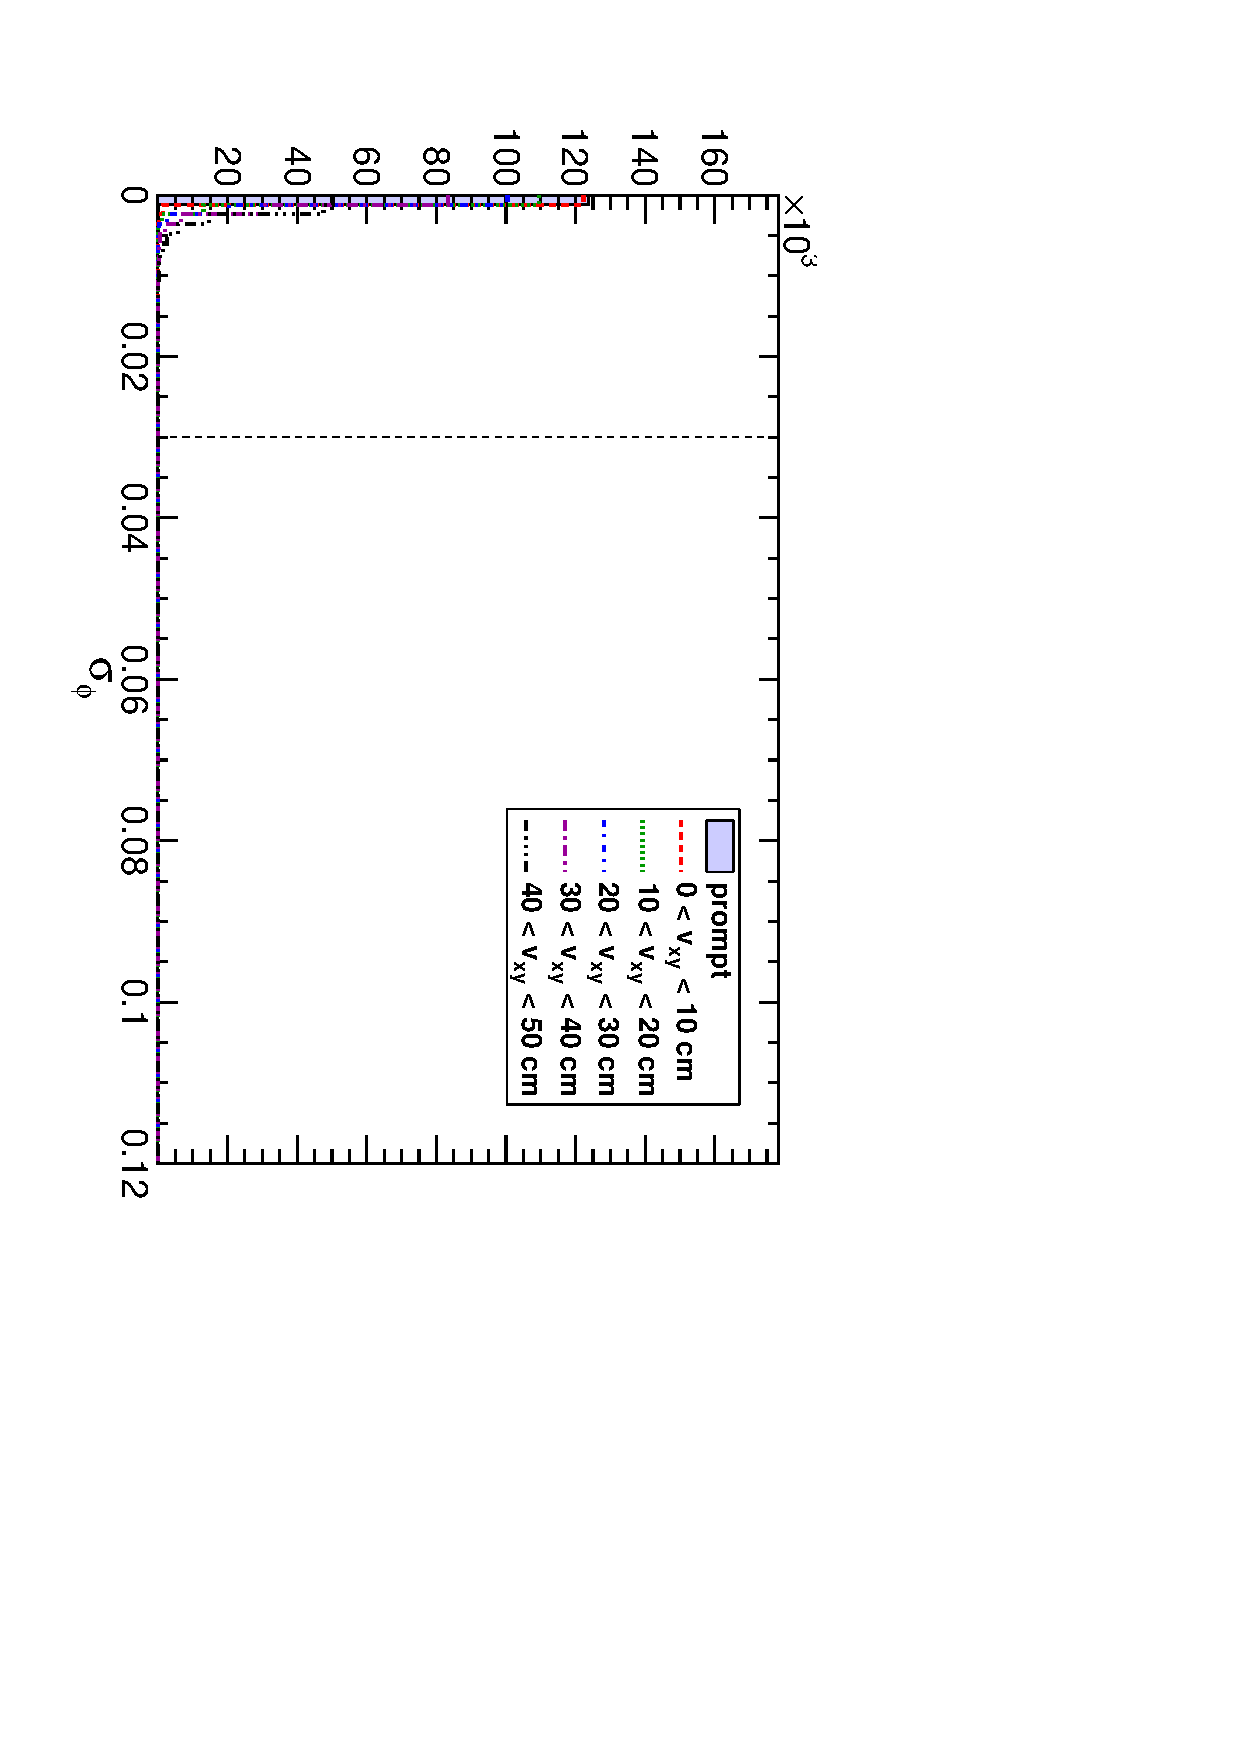
\includegraphics[height=\linewidth, angle=90]{fig/backgrounds3_plot/trackslinear_phierr.pdf}
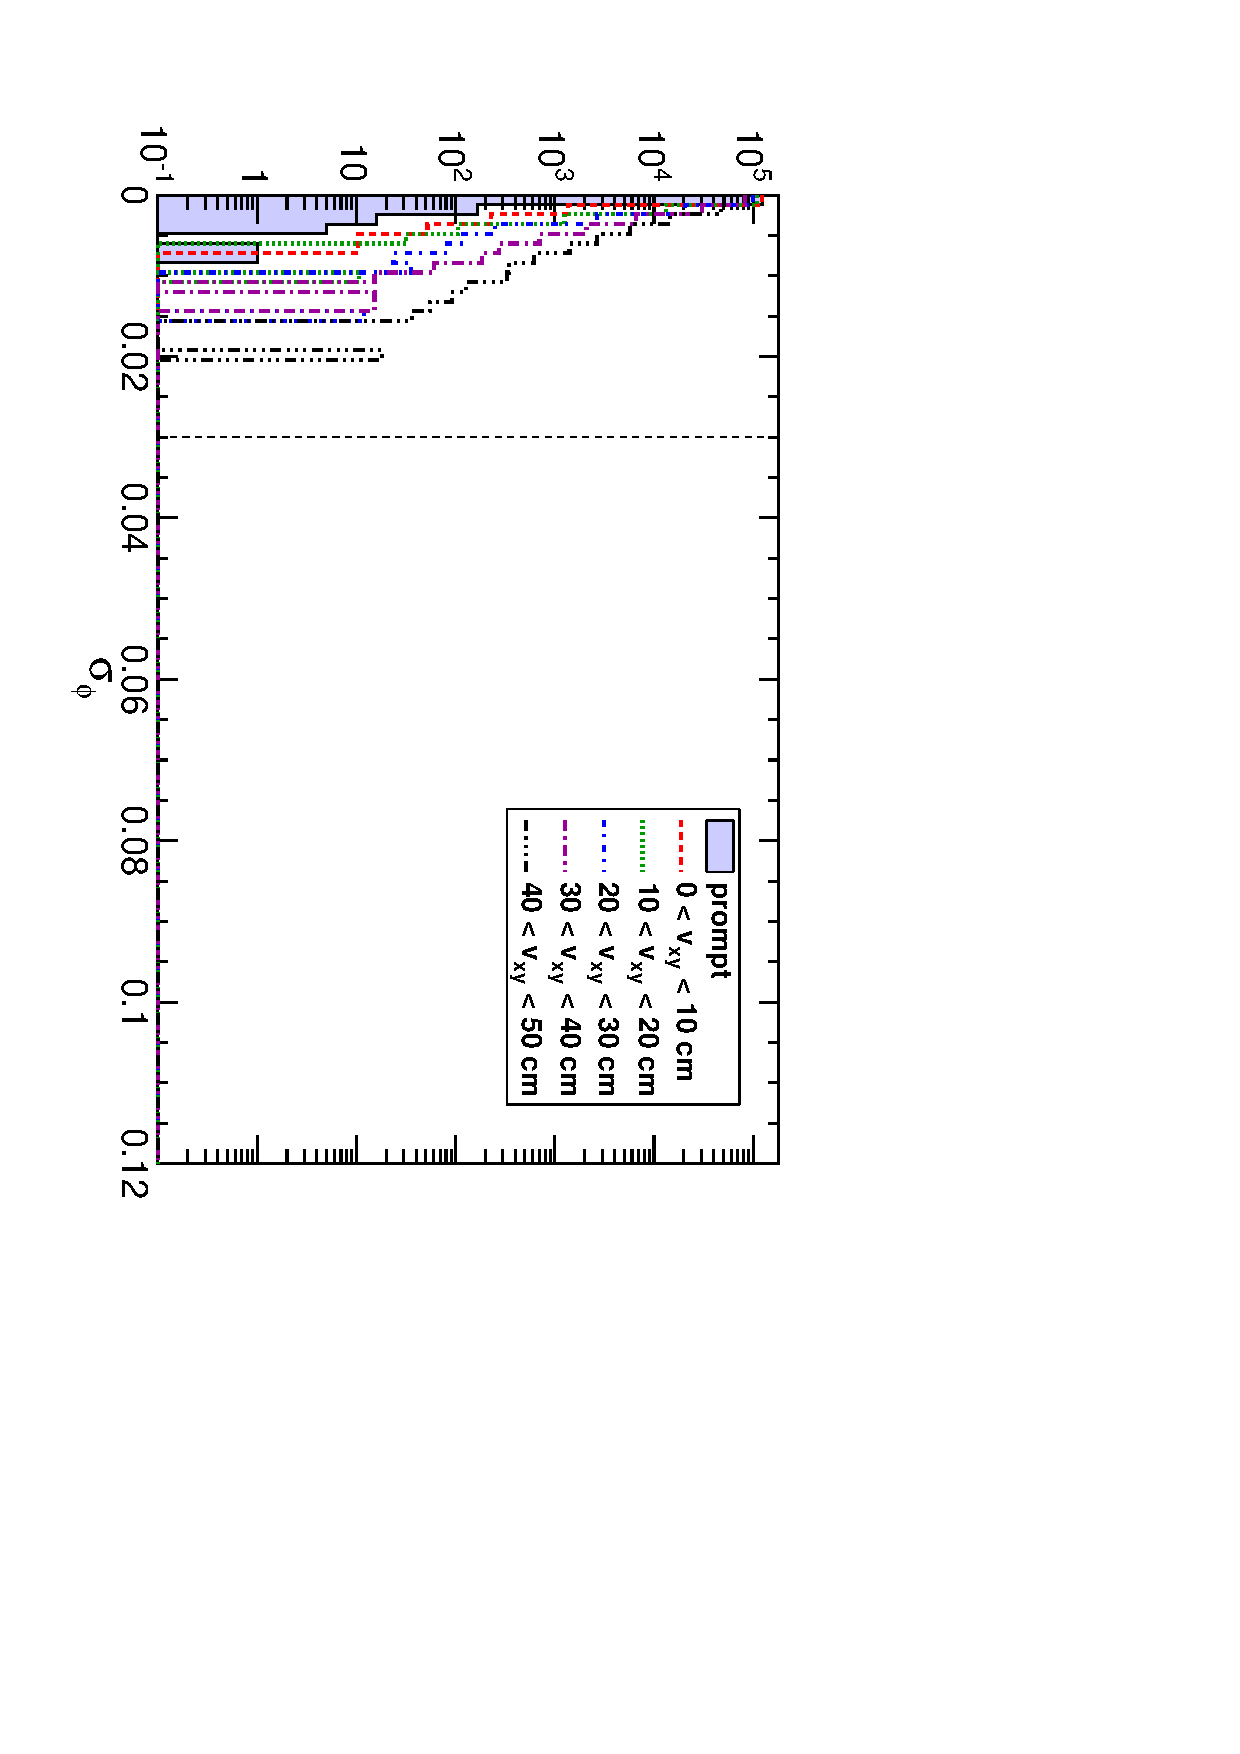
\includegraphics[height=\linewidth, angle=90]{fig/backgrounds3_plot/trackslog_phierr.pdf}
\end{multicols}

\caption{Performance of uncertainty in tracker $\phi$ cut.  Left: TrackerMuon (with $N_\s{segments}~\ge~2$) efficiency and backgrounds vs.\ $v_{xy}$ with the cut; right: linear and log distributions of the cut with the threshold indicated by a vertical line. \label{fig:phierr}}
\end{center}
\end{figure}

\begin{figure}
\begin{center}
\begin{multicols}{2}
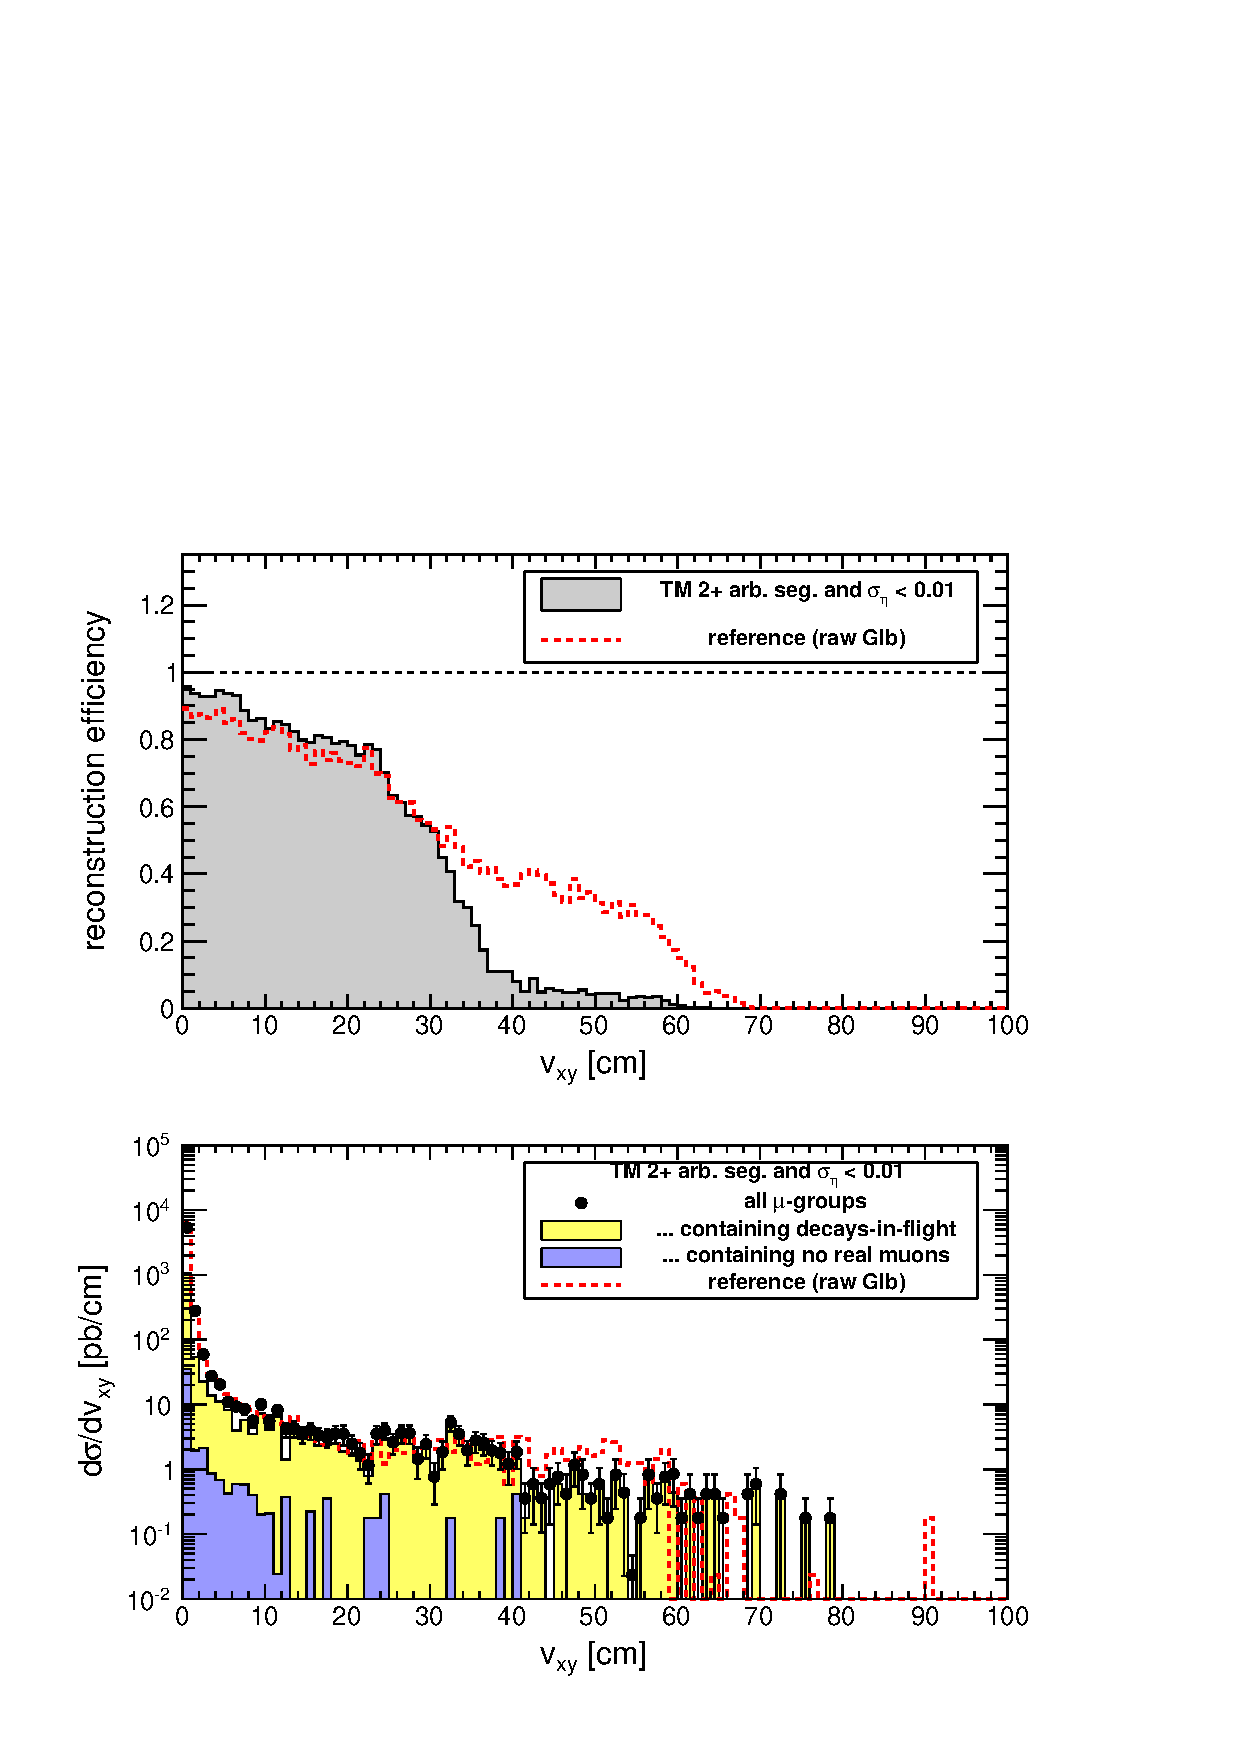
\includegraphics[width=\linewidth]{fig/backgrounds3_plot/dispvert_TrackerSegMatch2EtaErr.pdf}

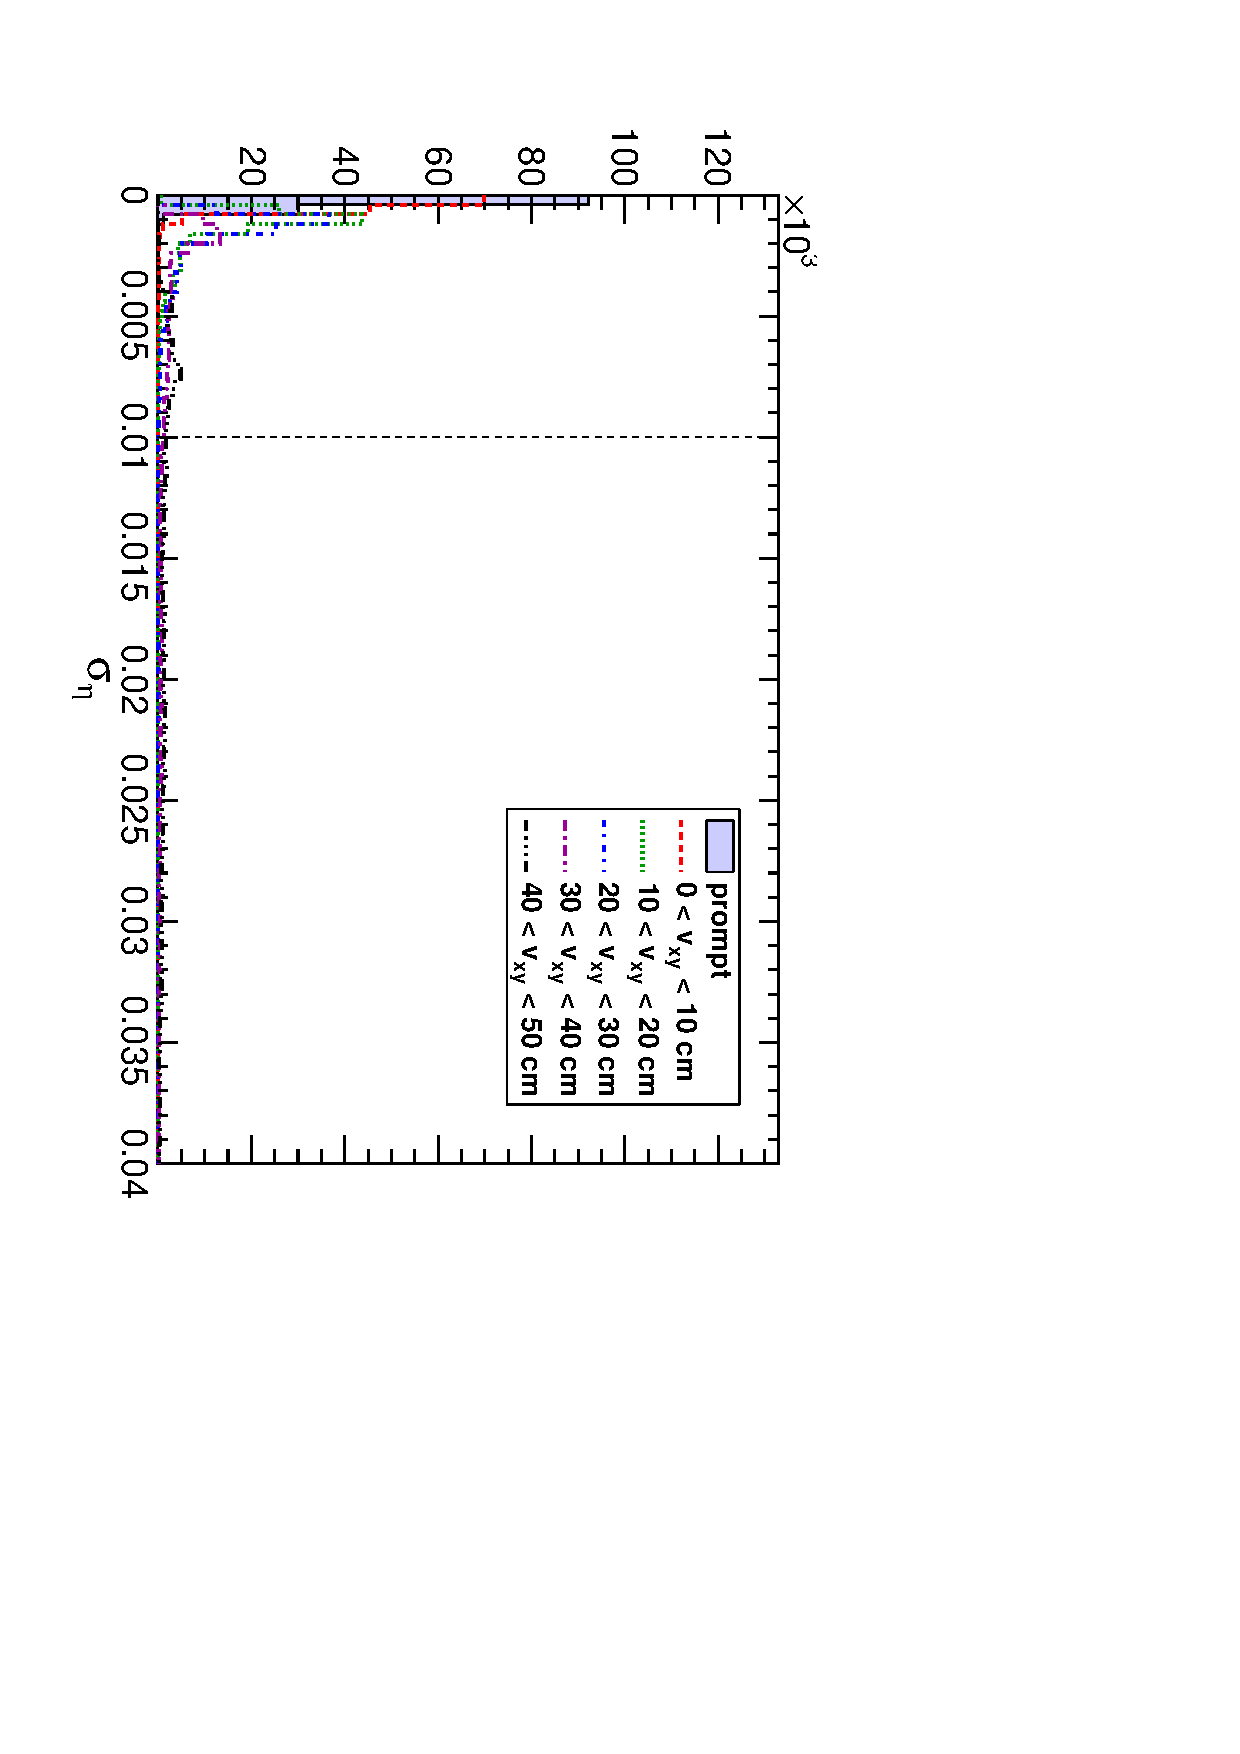
\includegraphics[height=\linewidth, angle=90]{fig/backgrounds3_plot/trackslinear_etaerr.pdf}
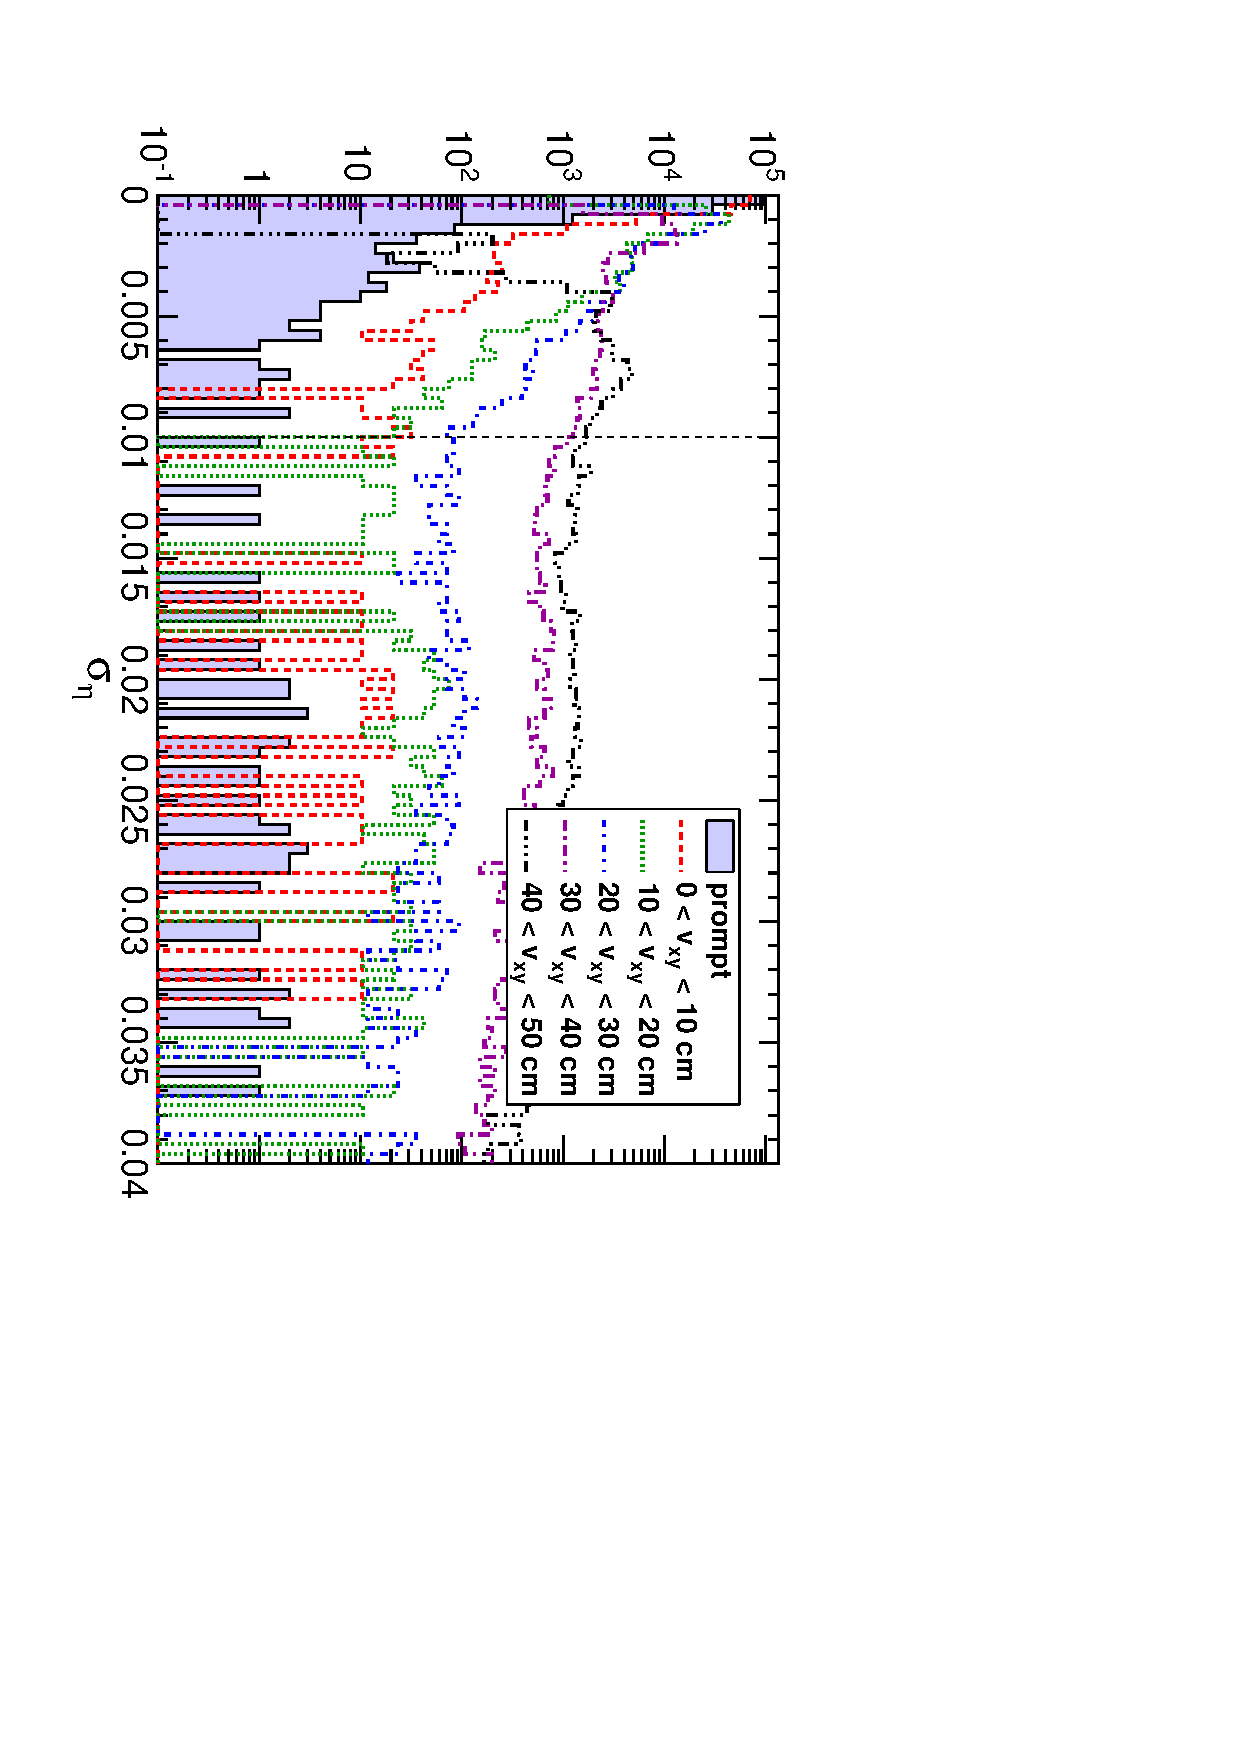
\includegraphics[height=\linewidth, angle=90]{fig/backgrounds3_plot/trackslog_etaerr.pdf}
\end{multicols}

\caption{Performance of uncertainty in tracker $\eta$ cut.  Left: TrackerMuon (with $N_\s{segments}~\ge~2$) efficiency and backgrounds vs.\ $v_{xy}$ with the cut; right: linear and log distributions of the cut with the threshold indicated by a vertical line. \label{fig:etaerr}}
\end{center}
\end{figure}

\begin{figure}
\begin{center}
\begin{multicols}{2}
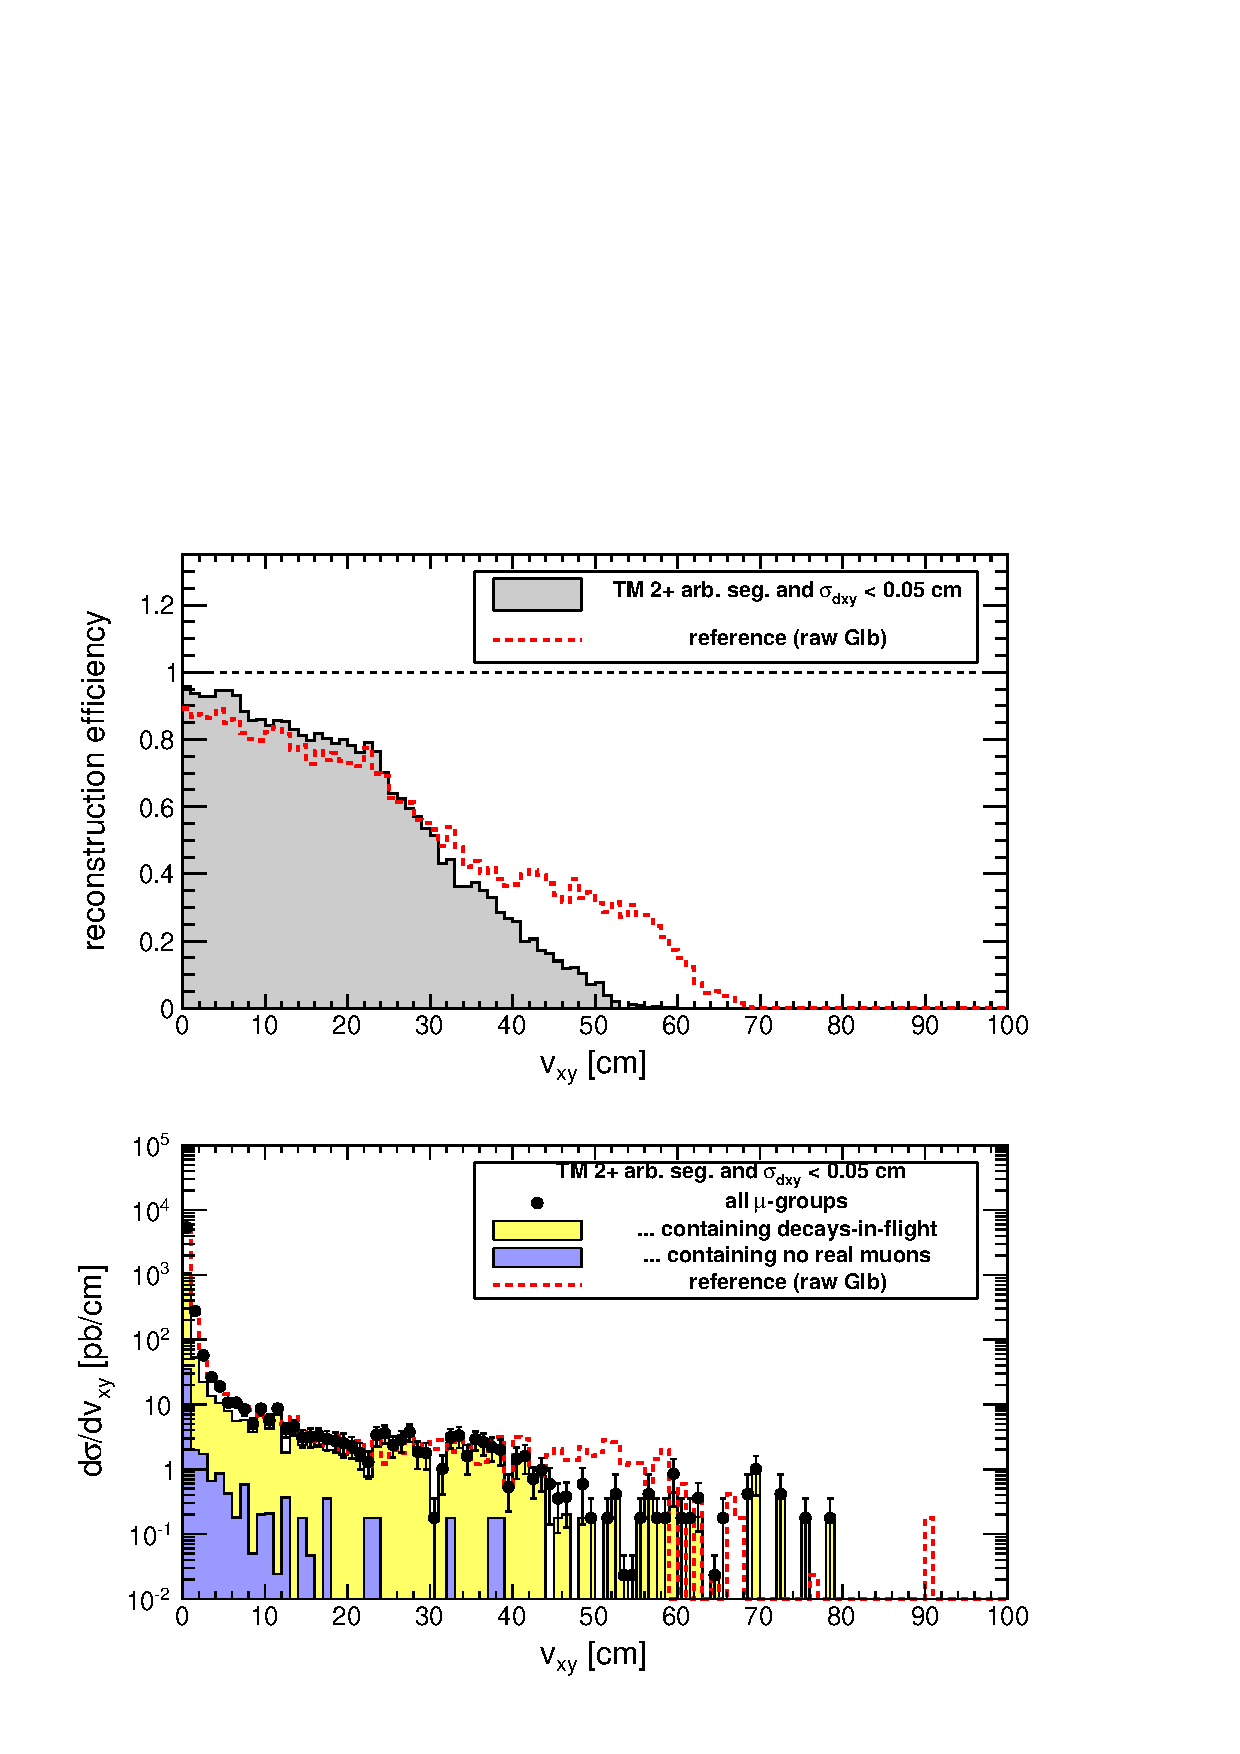
\includegraphics[width=\linewidth]{fig/backgrounds3_plot/dispvert_TrackerSegMatch2DxyErr.pdf}

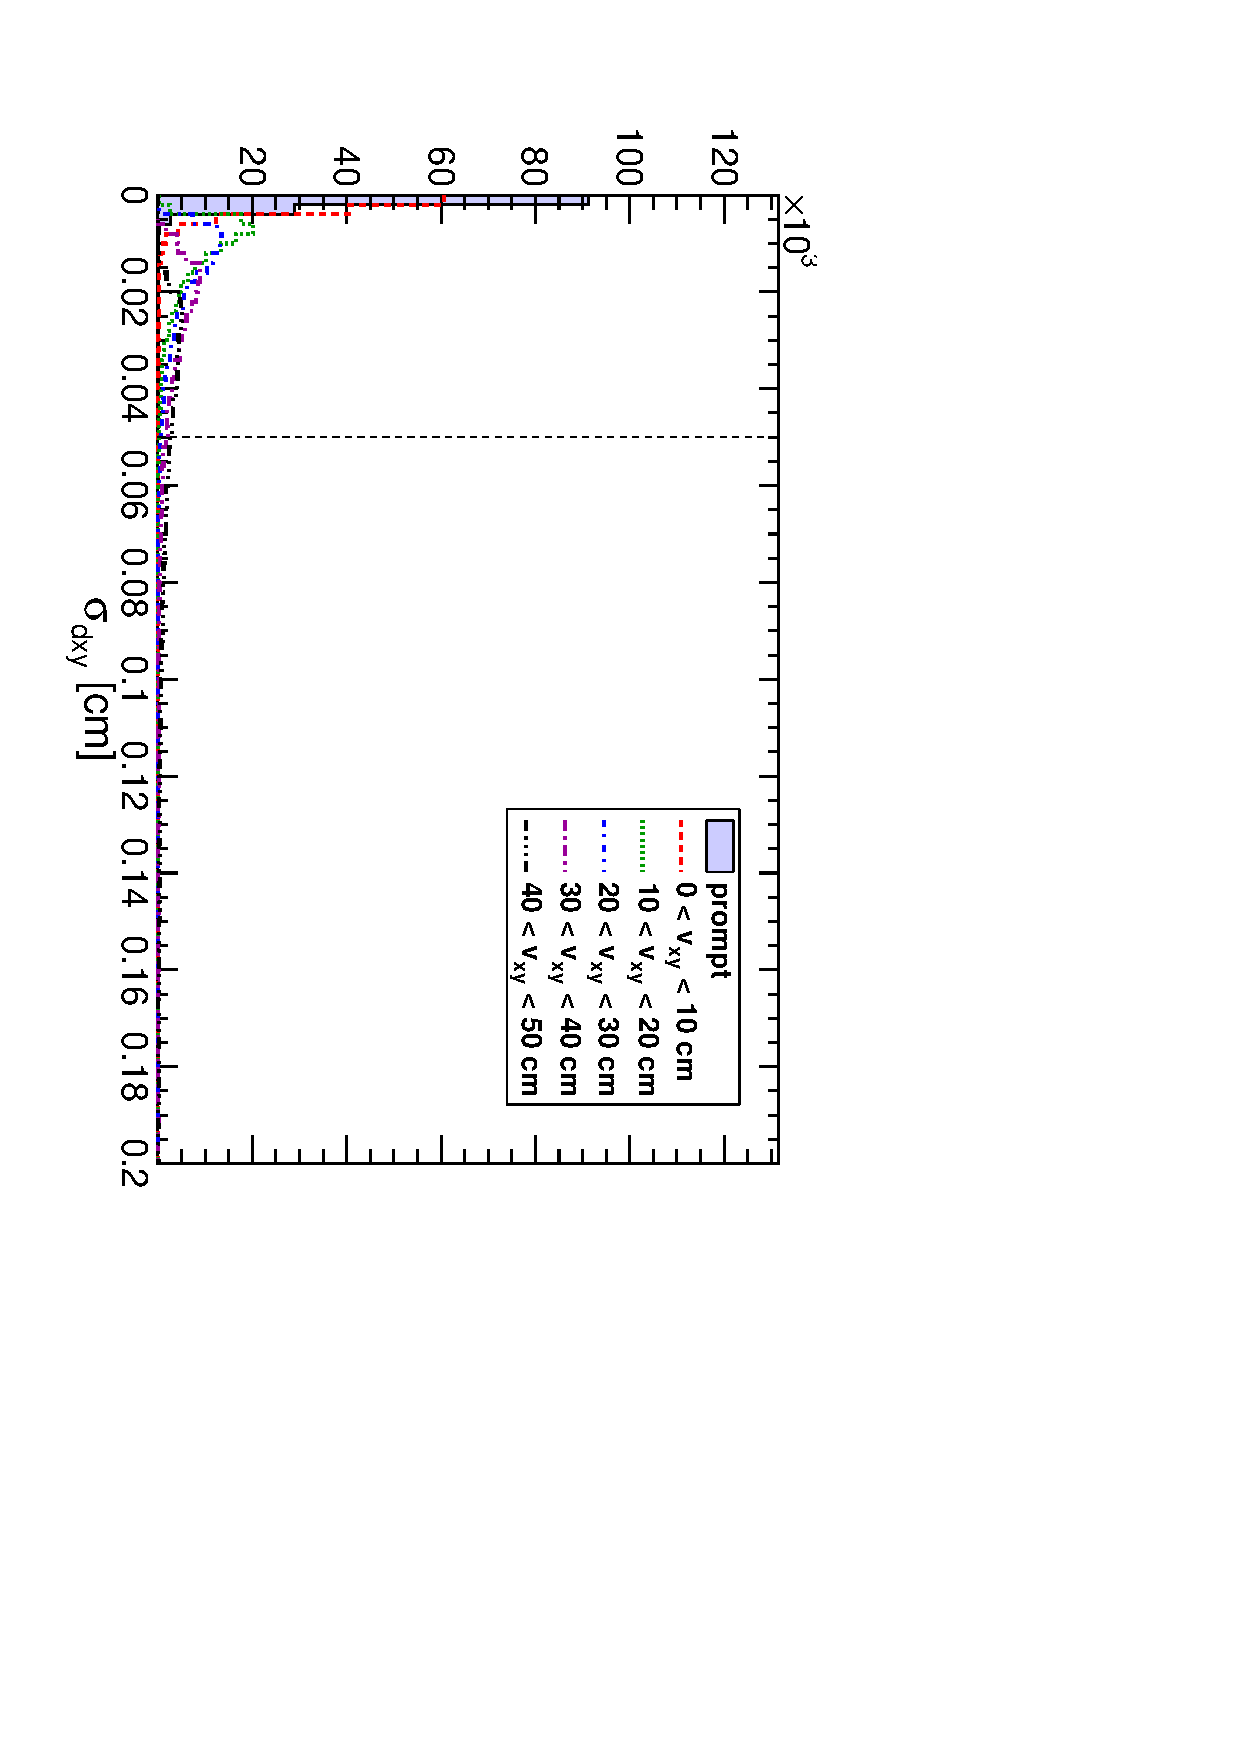
\includegraphics[height=\linewidth, angle=90]{fig/backgrounds3_plot/trackslinear_dxyerr.pdf}
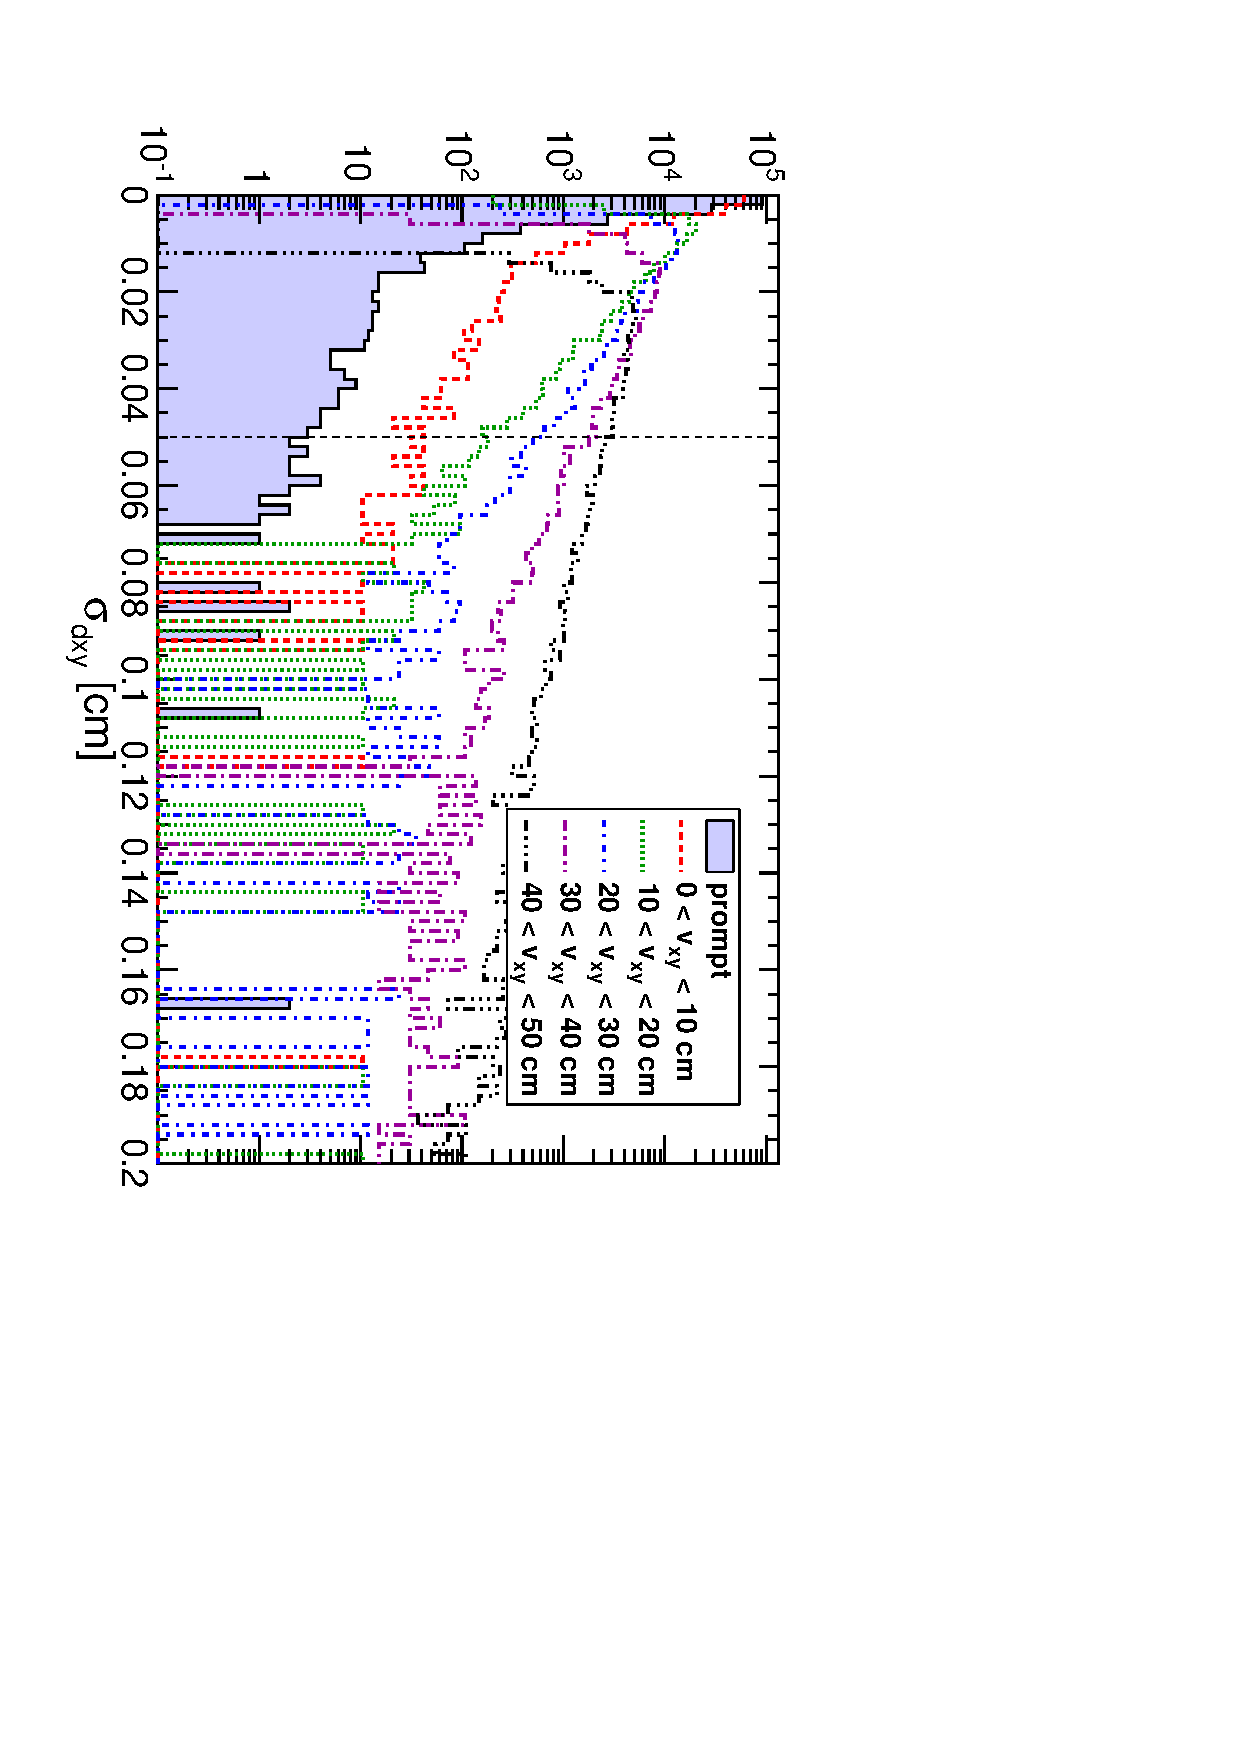
\includegraphics[height=\linewidth, angle=90]{fig/backgrounds3_plot/trackslog_dxyerr.pdf}
\end{multicols}

\caption{Performance of uncertainty in tracker $d_{xy}$ cut.  Left: TrackerMuon (with $N_\s{segments}~\ge~2$) efficiency and backgrounds vs.\ $v_{xy}$ with the cut; right: linear and log distributions of the cut with the threshold indicated by a vertical line. \label{fig:dxyerr}}
\end{center}
\end{figure}

\begin{figure}
\begin{center}
\begin{multicols}{2}
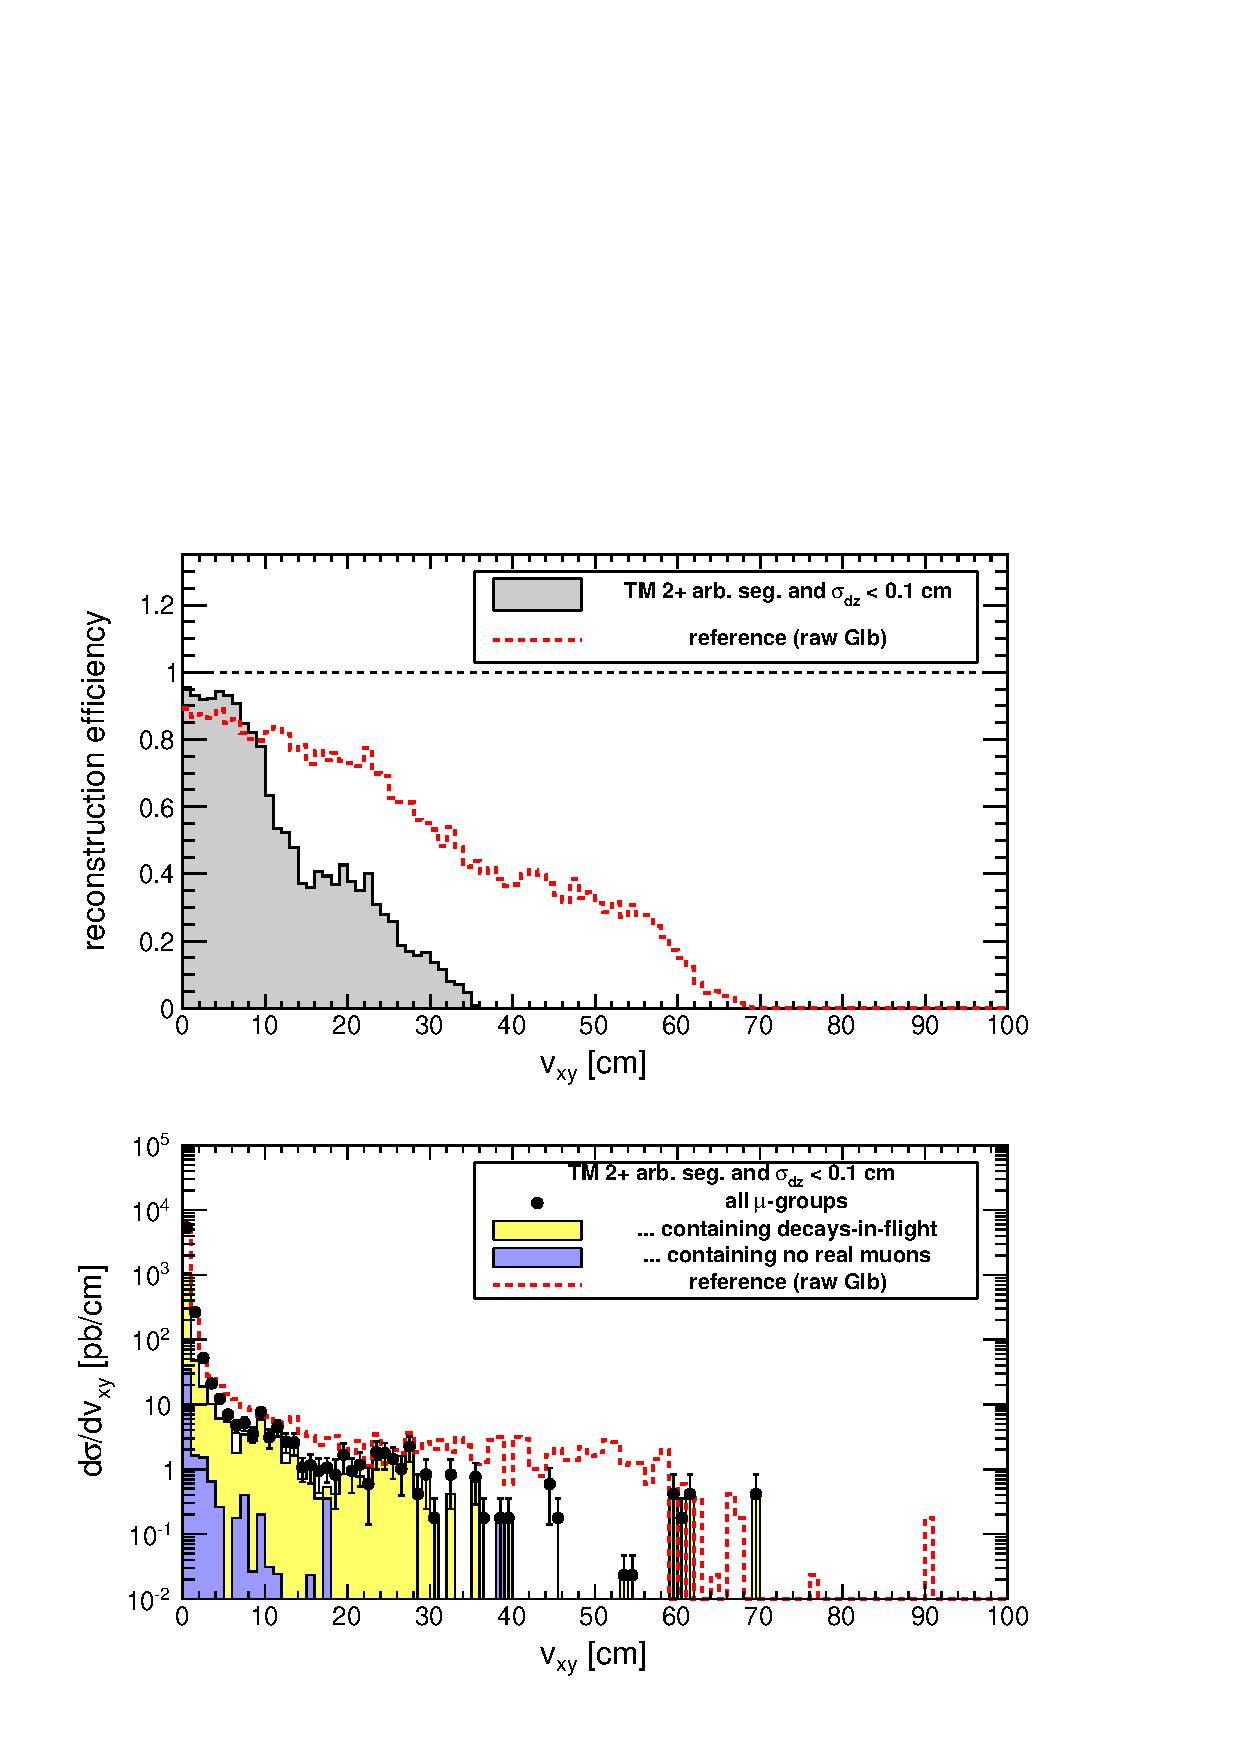
\includegraphics[width=\linewidth]{fig/backgrounds3_plot/dispvert_TrackerSegMatch2DzErr.pdf}

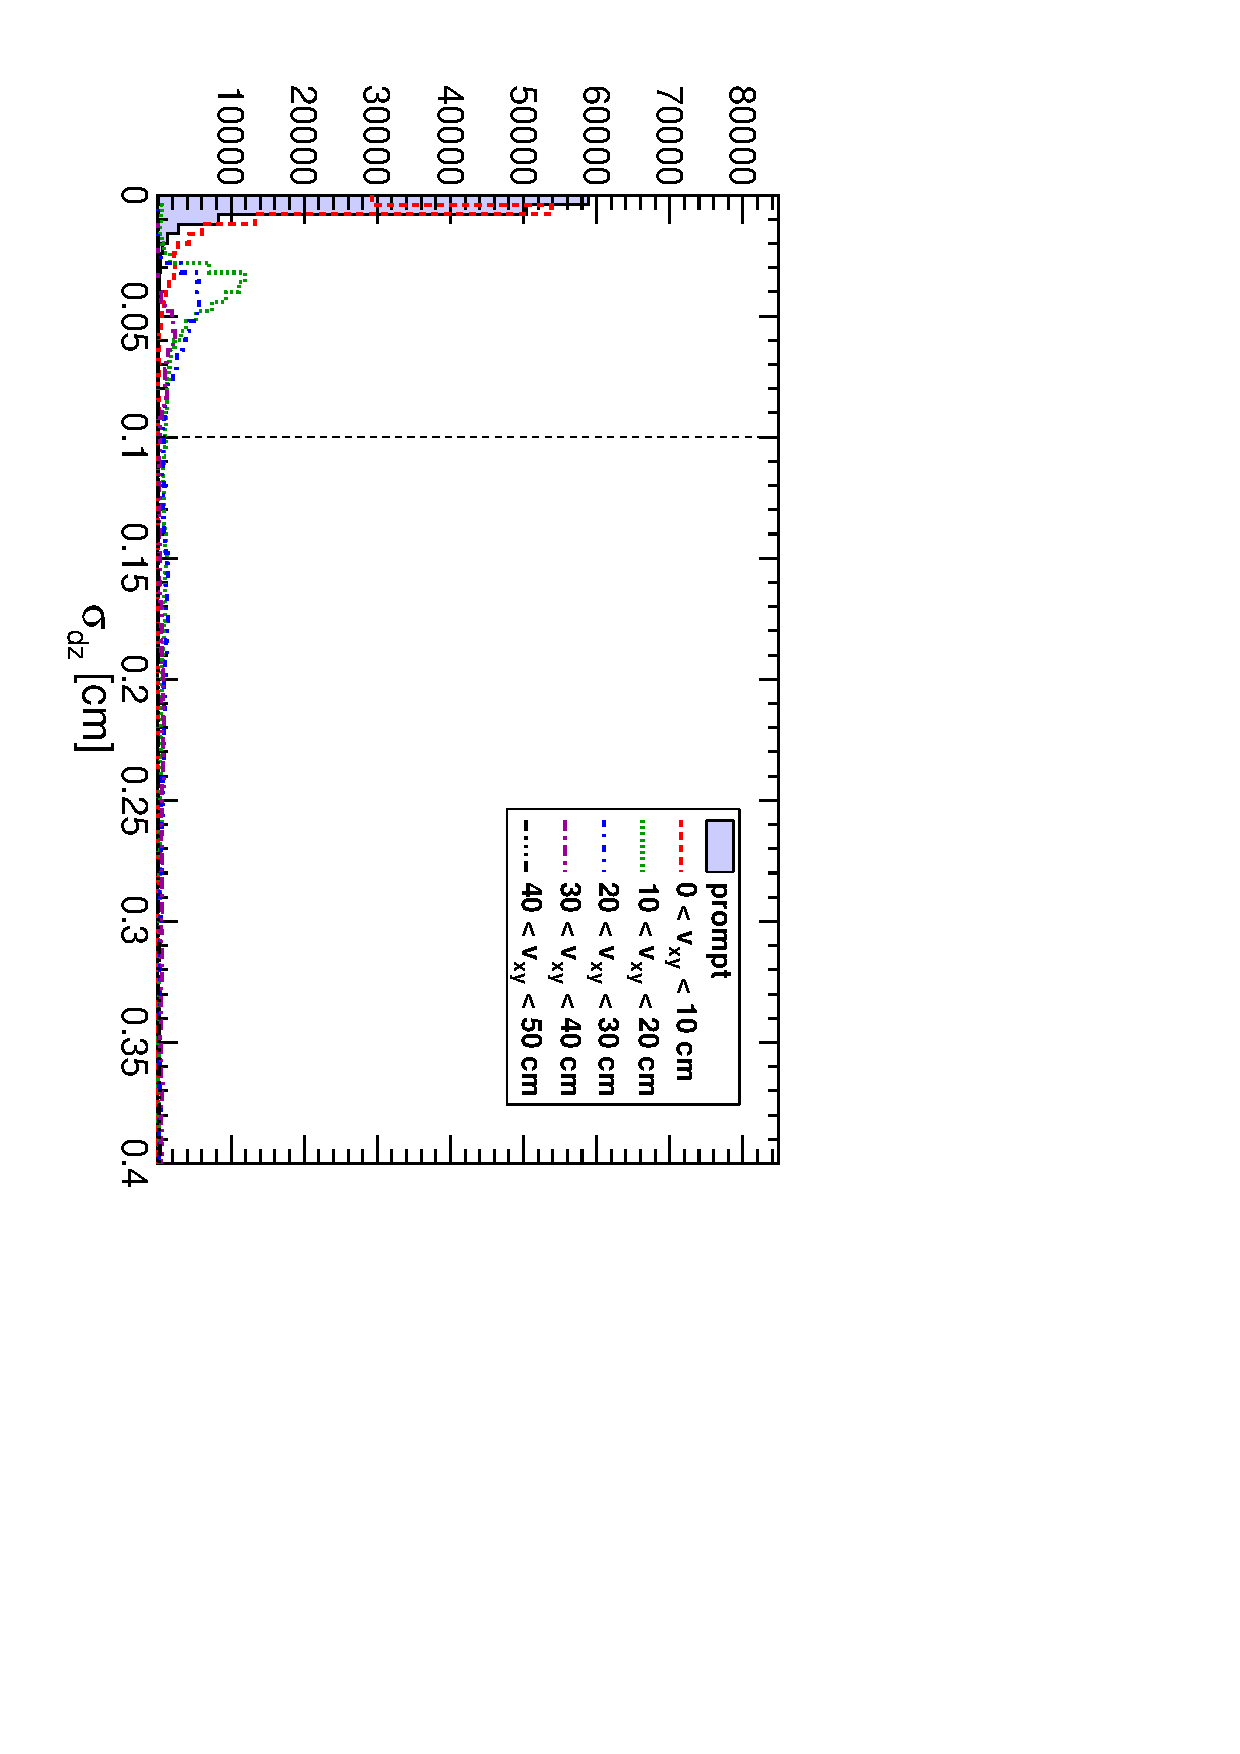
\includegraphics[height=\linewidth, angle=90]{fig/backgrounds3_plot/trackslinear_dzerr.pdf}
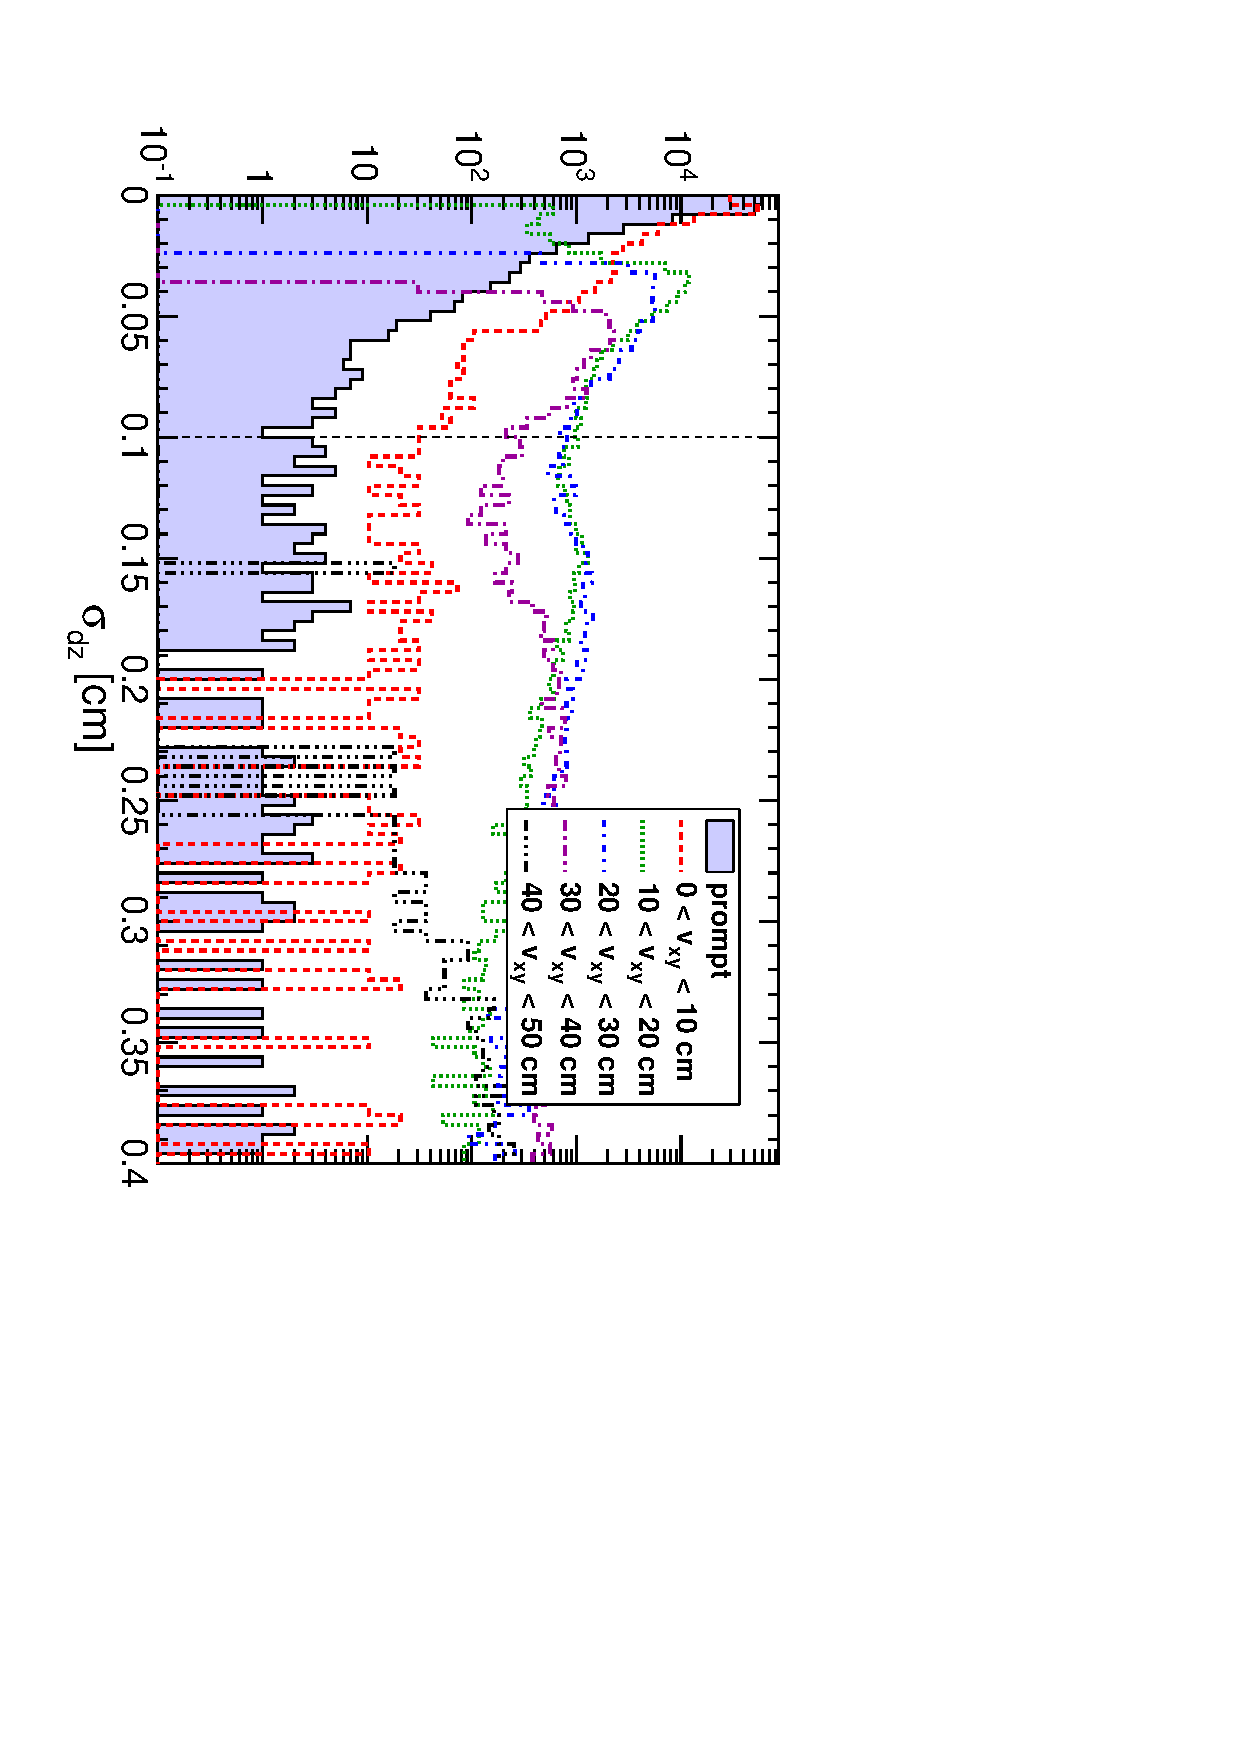
\includegraphics[height=\linewidth, angle=90]{fig/backgrounds3_plot/trackslog_dzerr.pdf}
\end{multicols}

\caption{Performance of uncertainty in tracker $d_z$ cut.  Left: TrackerMuon (with $N_\s{segments}~\ge~2$) efficiency and backgrounds vs.\ $v_{xy}$ with the cut; right: linear and log distributions of the cut with the threshold indicated by a vertical line. \label{fig:dzerr}}
\end{center}
\end{figure}

\clearpage
\section{Advertisement}

I've developed a set of tools for identifying and studying
multi-muons~\cite{mytools} that were designed with displaced vertices
in mind from the very beginning.  They use the same KalmanVertexFitter
as the $K_S$ and $\Lambda$-finding code (I learned about vertexing by
helping the Colorado group find the $\Xi$ cascade) but have the
additional advantage that multi-muons are identified as easily as
di-muons (one can always cut later).  If we used the same objects, it
would be easier to work together on characterizing the overlap of our
analyses (there's a continuum between prompt and displaced vertices).
The real work is in studying the physics and the detector, which
you've started; the software is just to make it more convenient to do
so.

I should also point out that the SVN repository\cite{svn} has a custom
particle gun MC generator ({\tt IOMC/ParticleGuns/src/MultiParticleByMassGunProducer.cc})
that produces events uniformly distributed in mass, $p_T$, and most
importantly (for you) $v_{xy}$.  This makes it easier to do
object-level efficiency and resolution studies.

\section{Conclusions?}

Not really.  Good luck!

\begin{thebibliography}{99}

\bibitem{strassler}
  \href{http://www.physics.rutgers.edu/~strassler/hv/hv.htm}{\tt http://www.physics.rutgers.edu/$\sim$strassler/hv/hv.htm}

\bibitem{geant}
  \href{http://geant4.cern.ch/G4UsersDocuments/UsersGuides/PhysicsReferenceManual/html/node28.html}{\tt
    http://geant4.cern.ch/G4UsersDocuments/UsersGuides/ PhysicsReferenceManual/html/node28.html}

\bibitem{conversions_tracking}
  \href{https://twiki.cern.ch/twiki//bin/view/CMS/TRK10003DedicatedTracking}{\tt https://twiki.cern.ch/twiki//bin/view/CMS/TRK10003DedicatedTracking}

\bibitem{mytools}
  \href{https://twiki.cern.ch/twiki/bin/view/CMS/ExoticaMuonJets}{\tt https://twiki.cern.ch/twiki/bin/view/CMS/ExoticaMuonJets}

\bibitem{svn}
  \href{https://svnweb.cern.ch/cern/wsvn/LeJOG/trunk/}{\tt https://svnweb.cern.ch/cern/wsvn/LeJOG/trunk/}

\end{thebibliography}

\end{document}
